\chapter{Rezepte} \label{ch:appendix_rezepte}
\vspace{-1.0\baselineskip}

Die sind die Rezepte mit den Mengenangaben. Dabei wurde Packpulver mit dem Faktor $0,75$ in Natron umgerechnet.
Zudem wurden sämtliche Zutaten, die als Füllung gedacht sind mit SchokoSt bezeichnet.
Zucker jeglicher Art (raffinierter, braun oder Vanillezucker) wurde zu Zucker hinzugezählt.
War bei den Zutaten von einem Eigelb die Rede wird dieses mit als $0,5$\,Eier gewertet.  
\begin{table}[h!]
\centering
\caption{Rezepte mit Mengenangabe der Zutaten (Teil 1: Basisteig)}
\label{table:rezepte_1}
\begin{tabular}{|l|r|r|r|r|}
\hline
Rezept & Mehl (g) & Butter (g) & Zucker (g) & Eier (Stk.) \\
\hline
R1     & 280      & 250        & 260        & 2,0         \\
R2     & 280      & 250        & 238        & 2,0         \\
R3     & 250      & 170        & 168        & 1,5         \\
R4     & 280      & 170        & 258        & 1,5         \\
R5     & 375      & 250        & 375        & 2,0         \\
R6     & 240      & 170        & 200        & 1,0         \\
R7     & 180      & 130        & 208        & 1,0         \\
R8     & 250      & 120        & 184        & 1,0         \\
\hline
\end{tabular}
\end{table}

\begin{table}[h!]
\centering
\caption{Rezepte mit Mengenangabe der Zutaten (Teil 2: Triebmittel und Schokost\"uckchen)}
\label{table:rezepte_2}
\begin{tabular}{|l|r|r|r|}
\hline
Rezept & Natron (g) & Salz (g) & SchokoSt (g) \\
\hline
R1     & 3,0        & 2,5      & 300          \\
R2     & 3,0        & 2,5      & 200          \\
R3     & 1,5        & 1,7      & 200          \\
R4     & 3,0        & 0,5      & 150          \\
R5     & 4,0        & 0,5      & 300          \\
R6     & 3,0        & 2,5      & 250          \\
R7     & 1,5        & 0,5      & 140          \\
R8     & 3,0        & 0,5      & 150          \\
\hline
\end{tabular}
\end{table}

% 1TL (gestr.) Salz entspricht 2,5 g
% 1TL Natron entspricht 3 g
% 1 Pck. Vanillezucker entspricht 8 g
% 1 TL Vanillezucker entspricht 4 g
% 1 Prise Salz entspricht 0,5 g
% Eier liegen meist bei 2 Stück
% Eier manchmal auch ein ganzen und ein Eigelb

% R1 : https://www.chefkoch.de/rezepte/2257651361176625/Subway-Cookies.html  
% R2 : https://www.chefkoch.de/rezepte/1378031243002711/American-Cookies-wie-bei-Subway.html  
% R3 : https://www.chefkoch.de/rezepte/470791140633601/Chewy-Chocolate-Chip-Cookies.html  
% R4 : https://www.chefkoch.de/rezepte/2601991408817771/American-Soft-Chocolate-Chip-Cookies.html  
% R5 : https://www.chefkoch.de/rezepte/614921161520963/World-s-best-Chocolate-Chip-Cookies.html  
% R6 : https://cookidoo.de/recipes/recipe/de-DE/r307943  
% R7 : https://cookidoo.de/recipes/recipe/de-DE/r47866    
% R8 : https://cookidoo.de/recipes/recipe/de-DE/r136546  


\begin{table}[H]
\centering
\caption{Links zu den Rezepten}
\label{table:rezepte_links}
\small
\begin{tabular}{|l|>{\RaggedRight\arraybackslash}p{0.78\textwidth}|}
\hline
Rezept & Link \\
\hline
R1     & \url{https://www.chefkoch.de/rezepte/2257651361176625/Subway-Cookies.html} \\
R2     & \url{https://www.chefkoch.de/rezepte/1378031243002711/American-Cookies-wie-bei-Subway.html} \\
R3     & \url{https://www.chefkoch.de/rezepte/470791140633601/Chewy-Chocolate-Chip-Cookies.html} \\
R4     & \url{https://www.chefkoch.de/rezepte/2601991408817771/American-Soft-Chocolate-Chip-Cookies.html} \\
R5     & \url{https://www.chefkoch.de/rezepte/614921161520963/World-s-best-Chocolate-Chip-Cookies.html} \\
R6     & \url{https://cookidoo.de/recipes/recipe/de-DE/r307943} \\
R7     & \url{https://cookidoo.de/recipes/recipe/de-DE/r47866} \\
R8     & \url{https://cookidoo.de/recipes/recipe/de-DE/r136546} \\
\hline
\end{tabular}
\end{table}



\chapter{Aufstellung der verwendeten Mess- und Prozessmittel} \label{ch:appendix_material}
\vspace{-1.0\baselineskip}
\begin{table}
\centering
\caption{Verwendete Messmittel}
\label{table:messmittel}
\begin{tabular}{|l|r|r|r|r|}
\hline
Messmittel        & Hersteller & Typ        & Auflösung & Beschreibung \\
\hline
Messschieber      & KRAFT      &            & 0,02mm    &               \\
Thermometer       &            &            && \\          
\hline
\end{tabular}
\end{table}

\begin{table}
\centering
\caption{Verwendete Prozessmittel}
\label{table:prozessmittel}
\begin{tabular}{|l|l|l|l|}
\hline
Prozessmittel     & Hersteller & Typ      & Beschreibung \\
Küchenwaage       & Tefal      &          &          \\
Feinwaage         &            &          &          \\
Thermomix         & Vorwerk    & TM6      &        \\
Vorratsbehälter   & IKEA       & IKEA 365+ Vorratsbehälter & mit luftdichten Kunstoffdeckel \\
Eisportionierer   & IKEA       & IDEALSIK & aus Edelstahl mit Doppellöffel   \\
\hline
\end{tabular}
\end{table}



\chapter{Cookies aus dem Vorversuch} \label{ch:appendix_vorversuch}
\vspace{-1.0\baselineskip}
\begin{figure}[H]
    \centering
    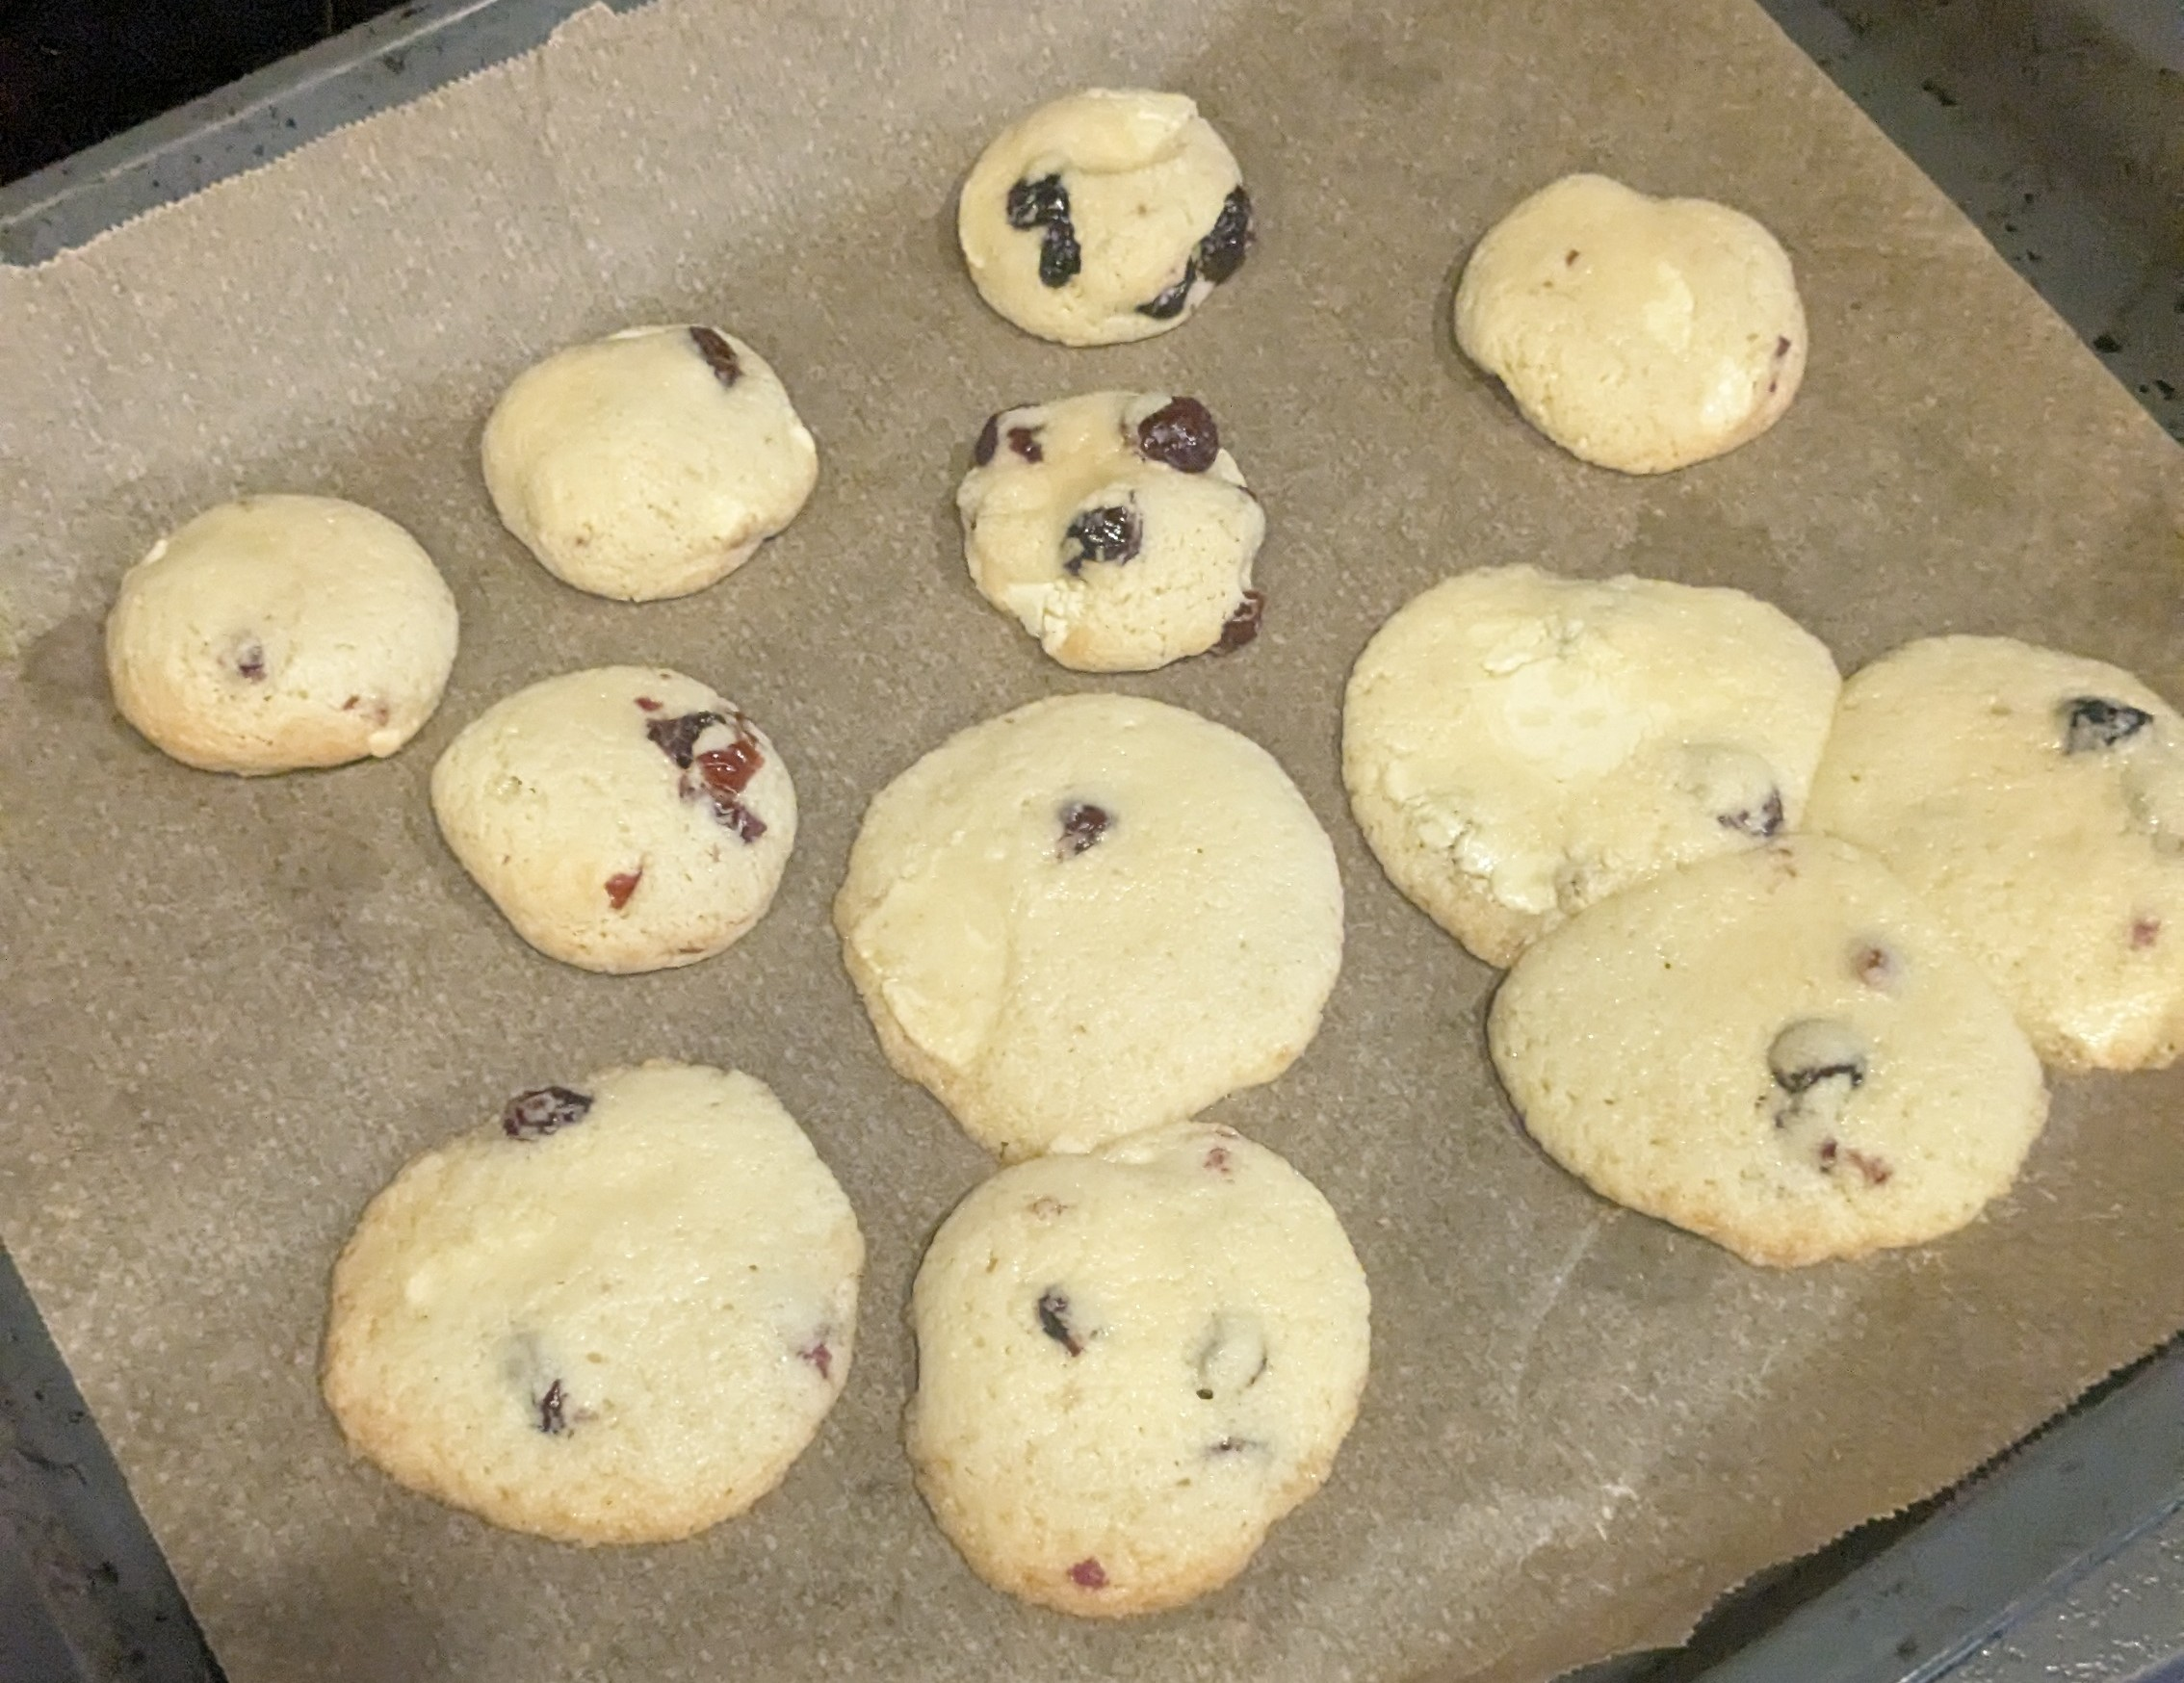
\includegraphics[width=\linewidth]{figures/vorversuch.jpg}
    \caption{Im Vorversuch mit unregelmäßigen Stücken von einer weißen Schokoladentafel und Cranberries ergaben sich variierende Cookie-Formen.}
    \label{fig:vorversuch}
\end{figure}

\chapter{Messmethoden} \label{ch:appendix_messung}
\vspace{-1.0\baselineskip}
\begin{figure}[H]
    \centering
    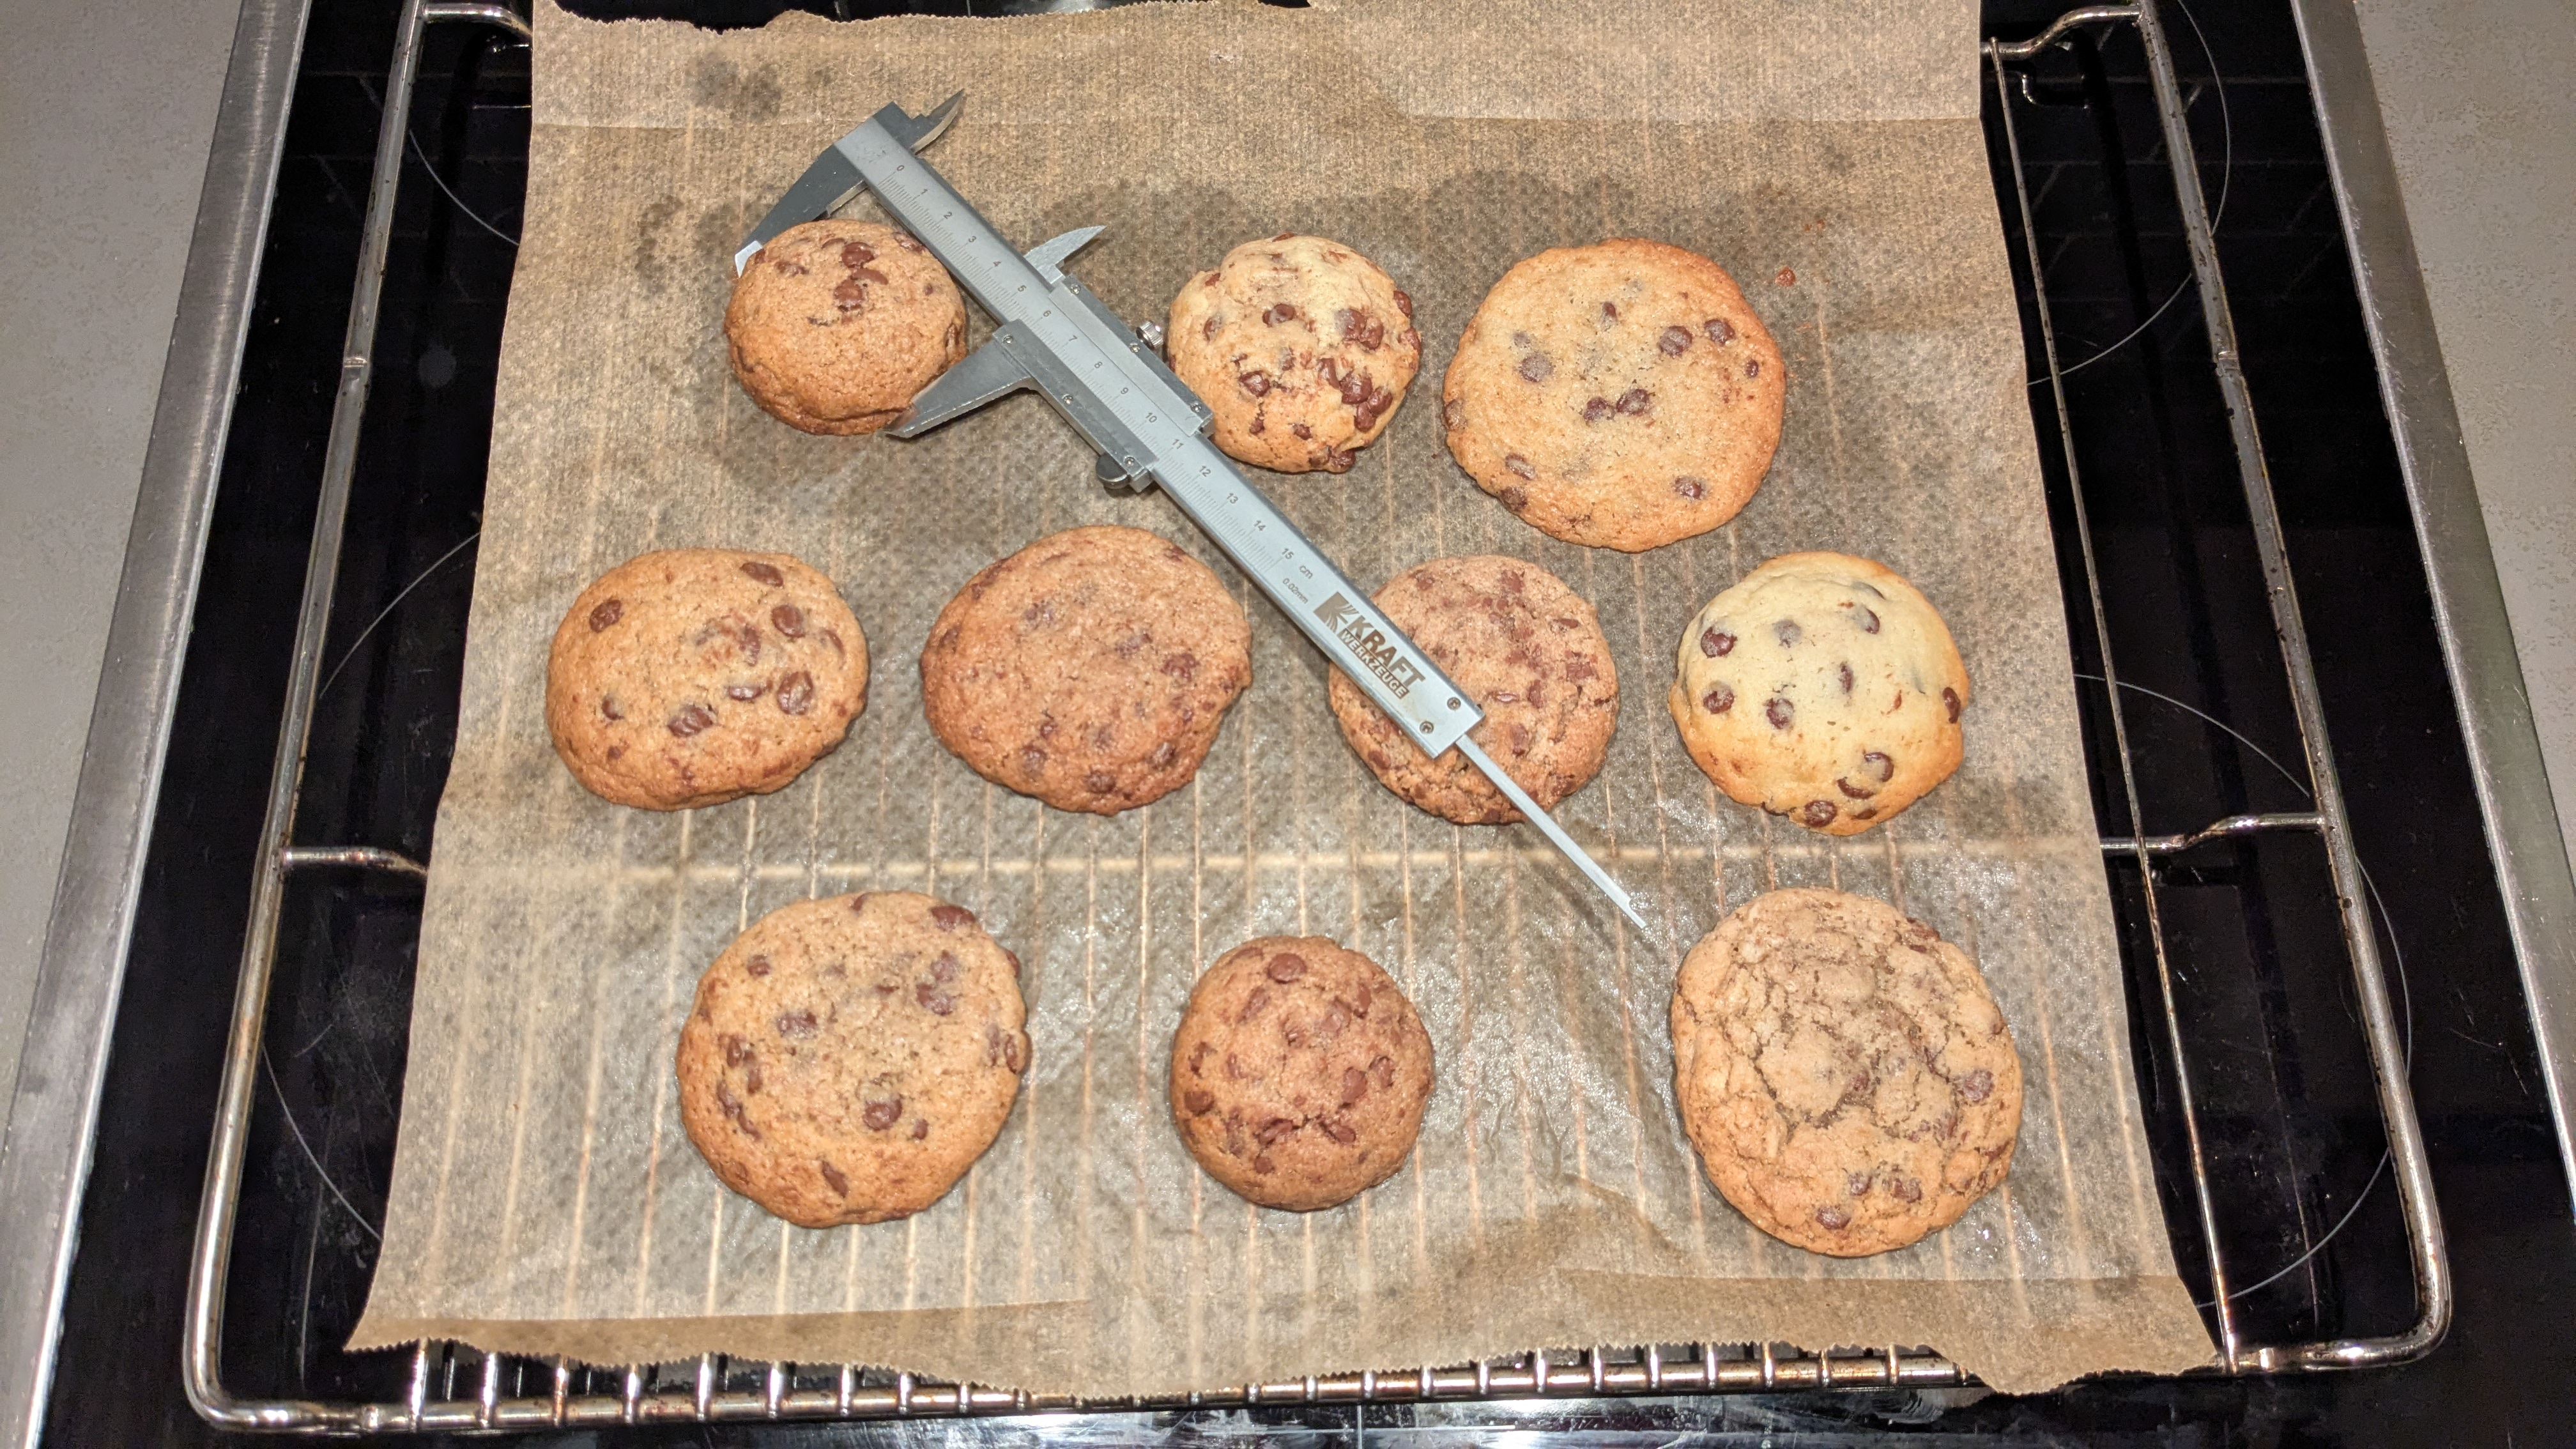
\includegraphics[width=\linewidth]{figures/messung_d1.jpg}
    \caption{Messung des ersten Durchmessers}
    \label{fig:messung_d1}
\end{figure}

\begin{figure}[H]
    \centering
    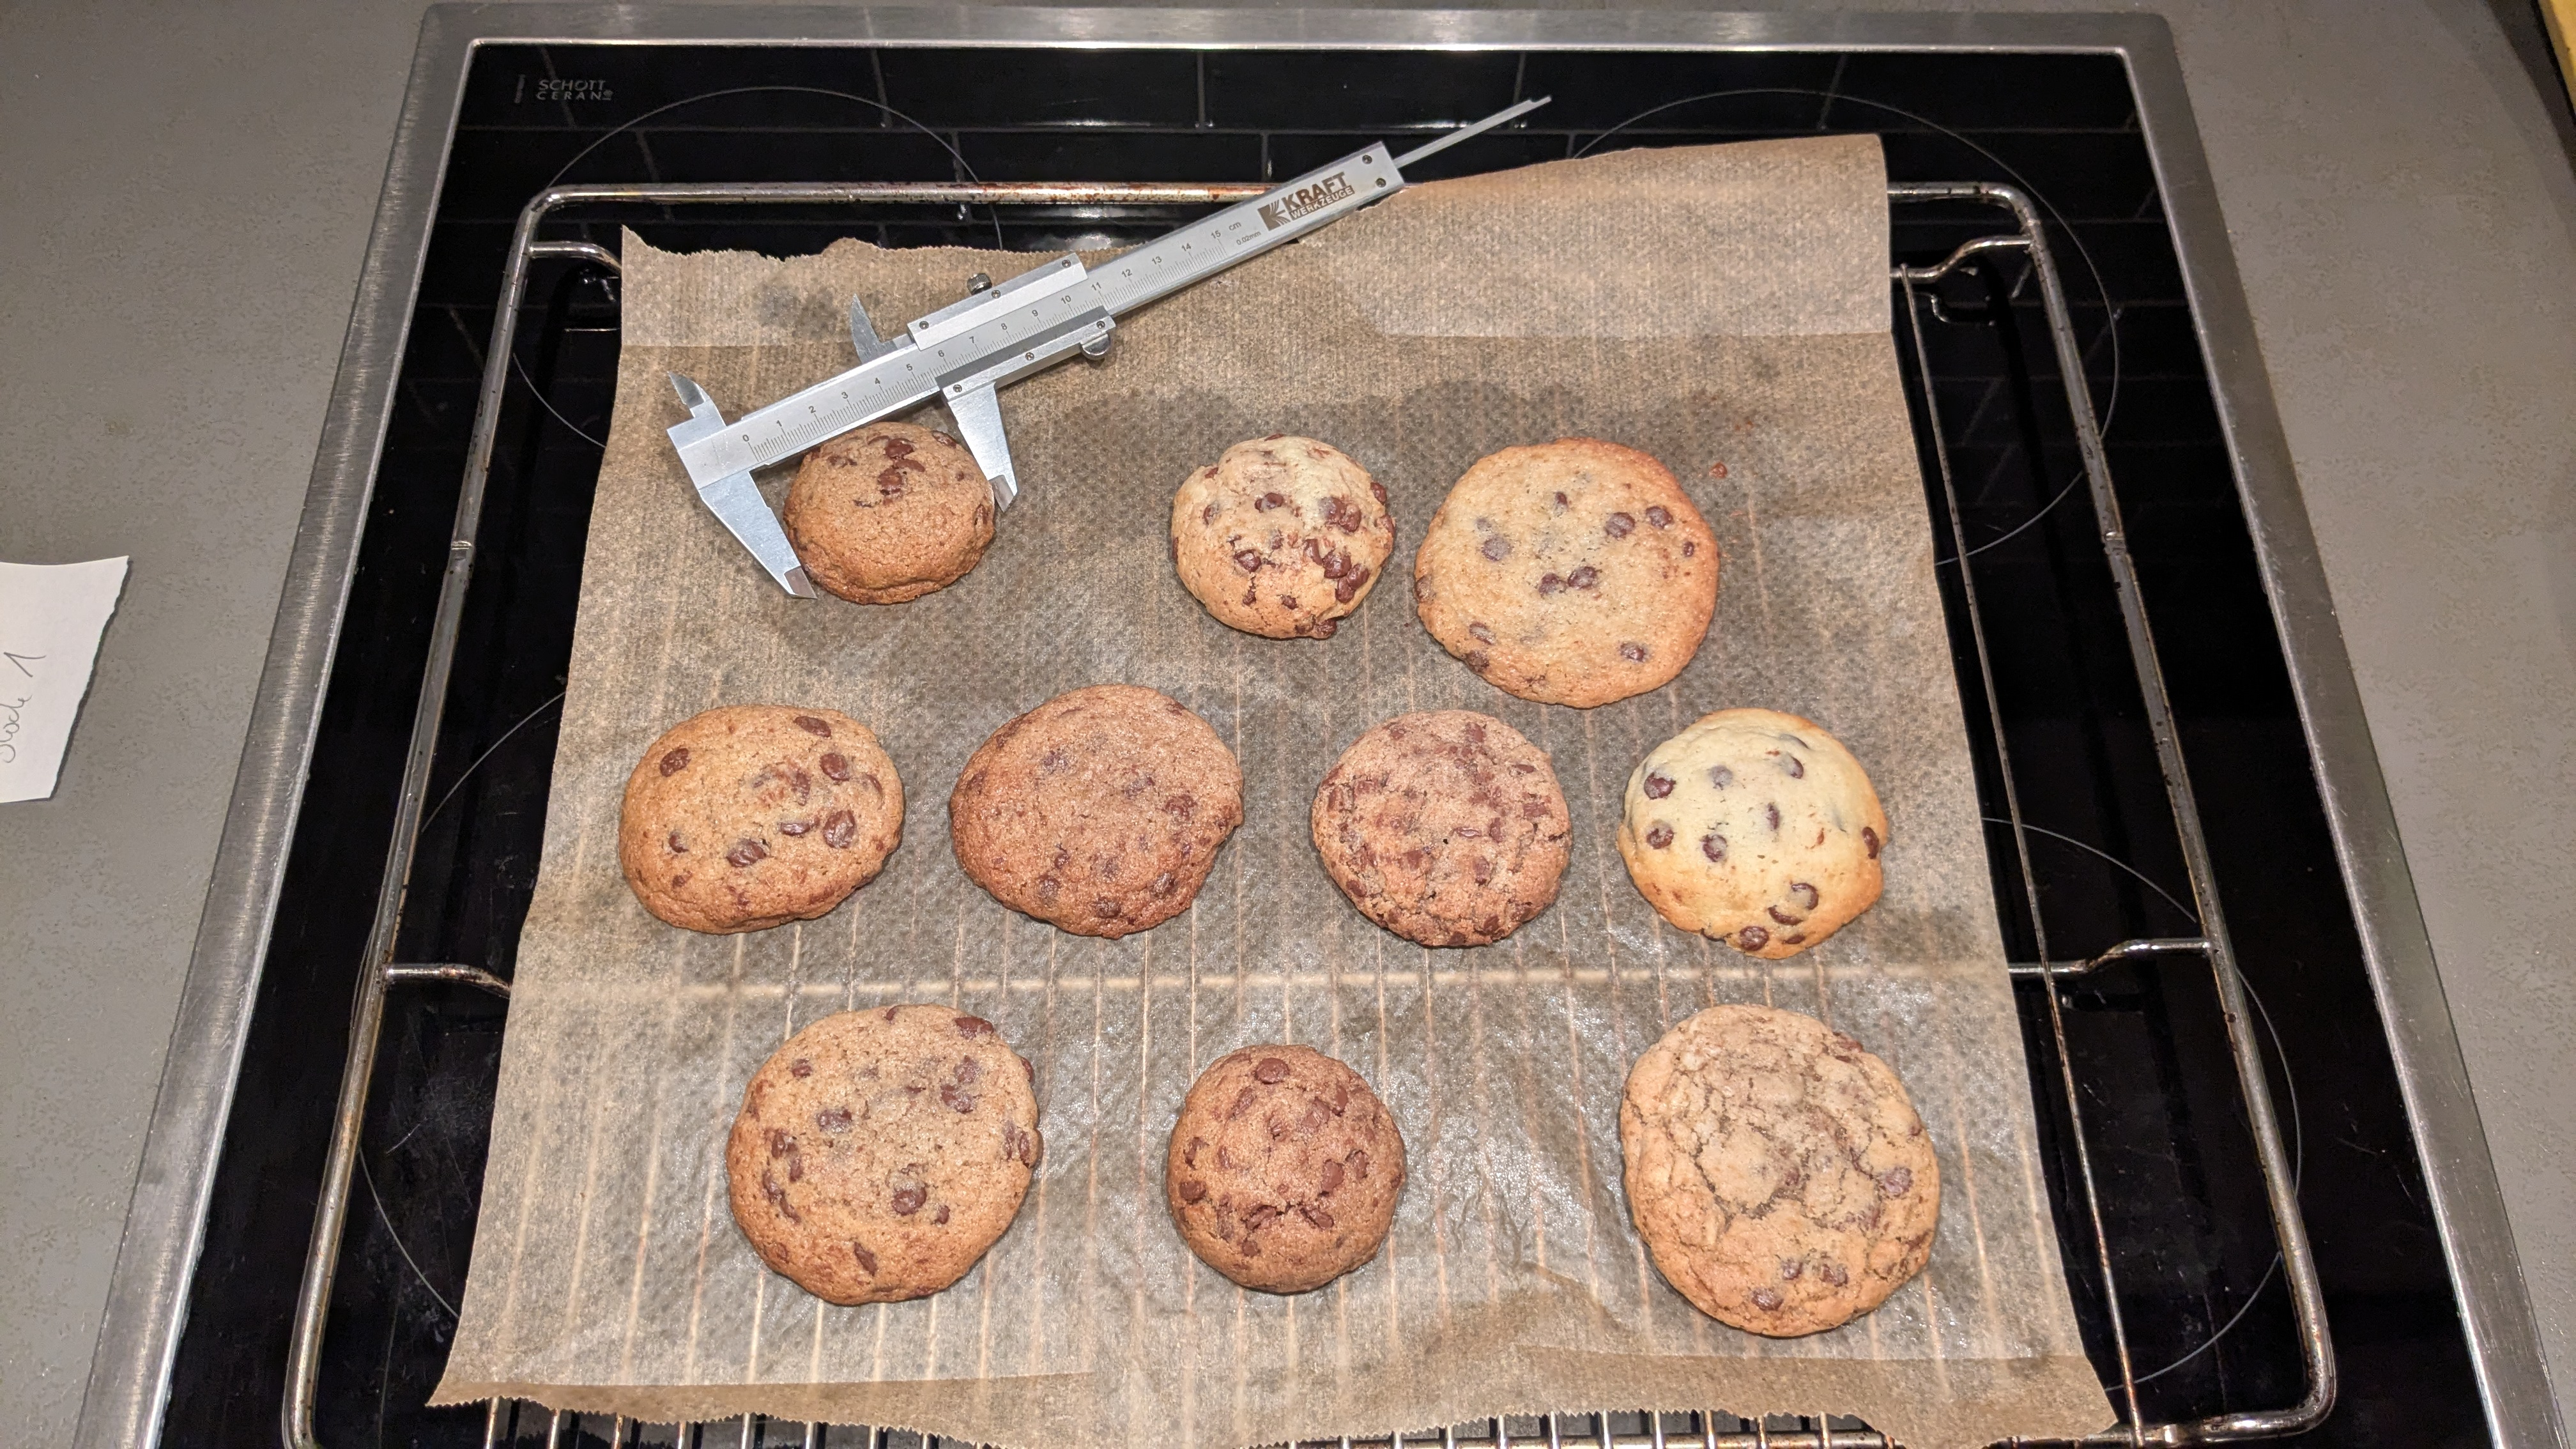
\includegraphics[width=\linewidth]{figures/messung_d2.jpg}
    \caption{Messung des zweiten Druchmessers}
    \label{fig:messung_d2}
\end{figure}

\begin{figure}[H]
    \centering
    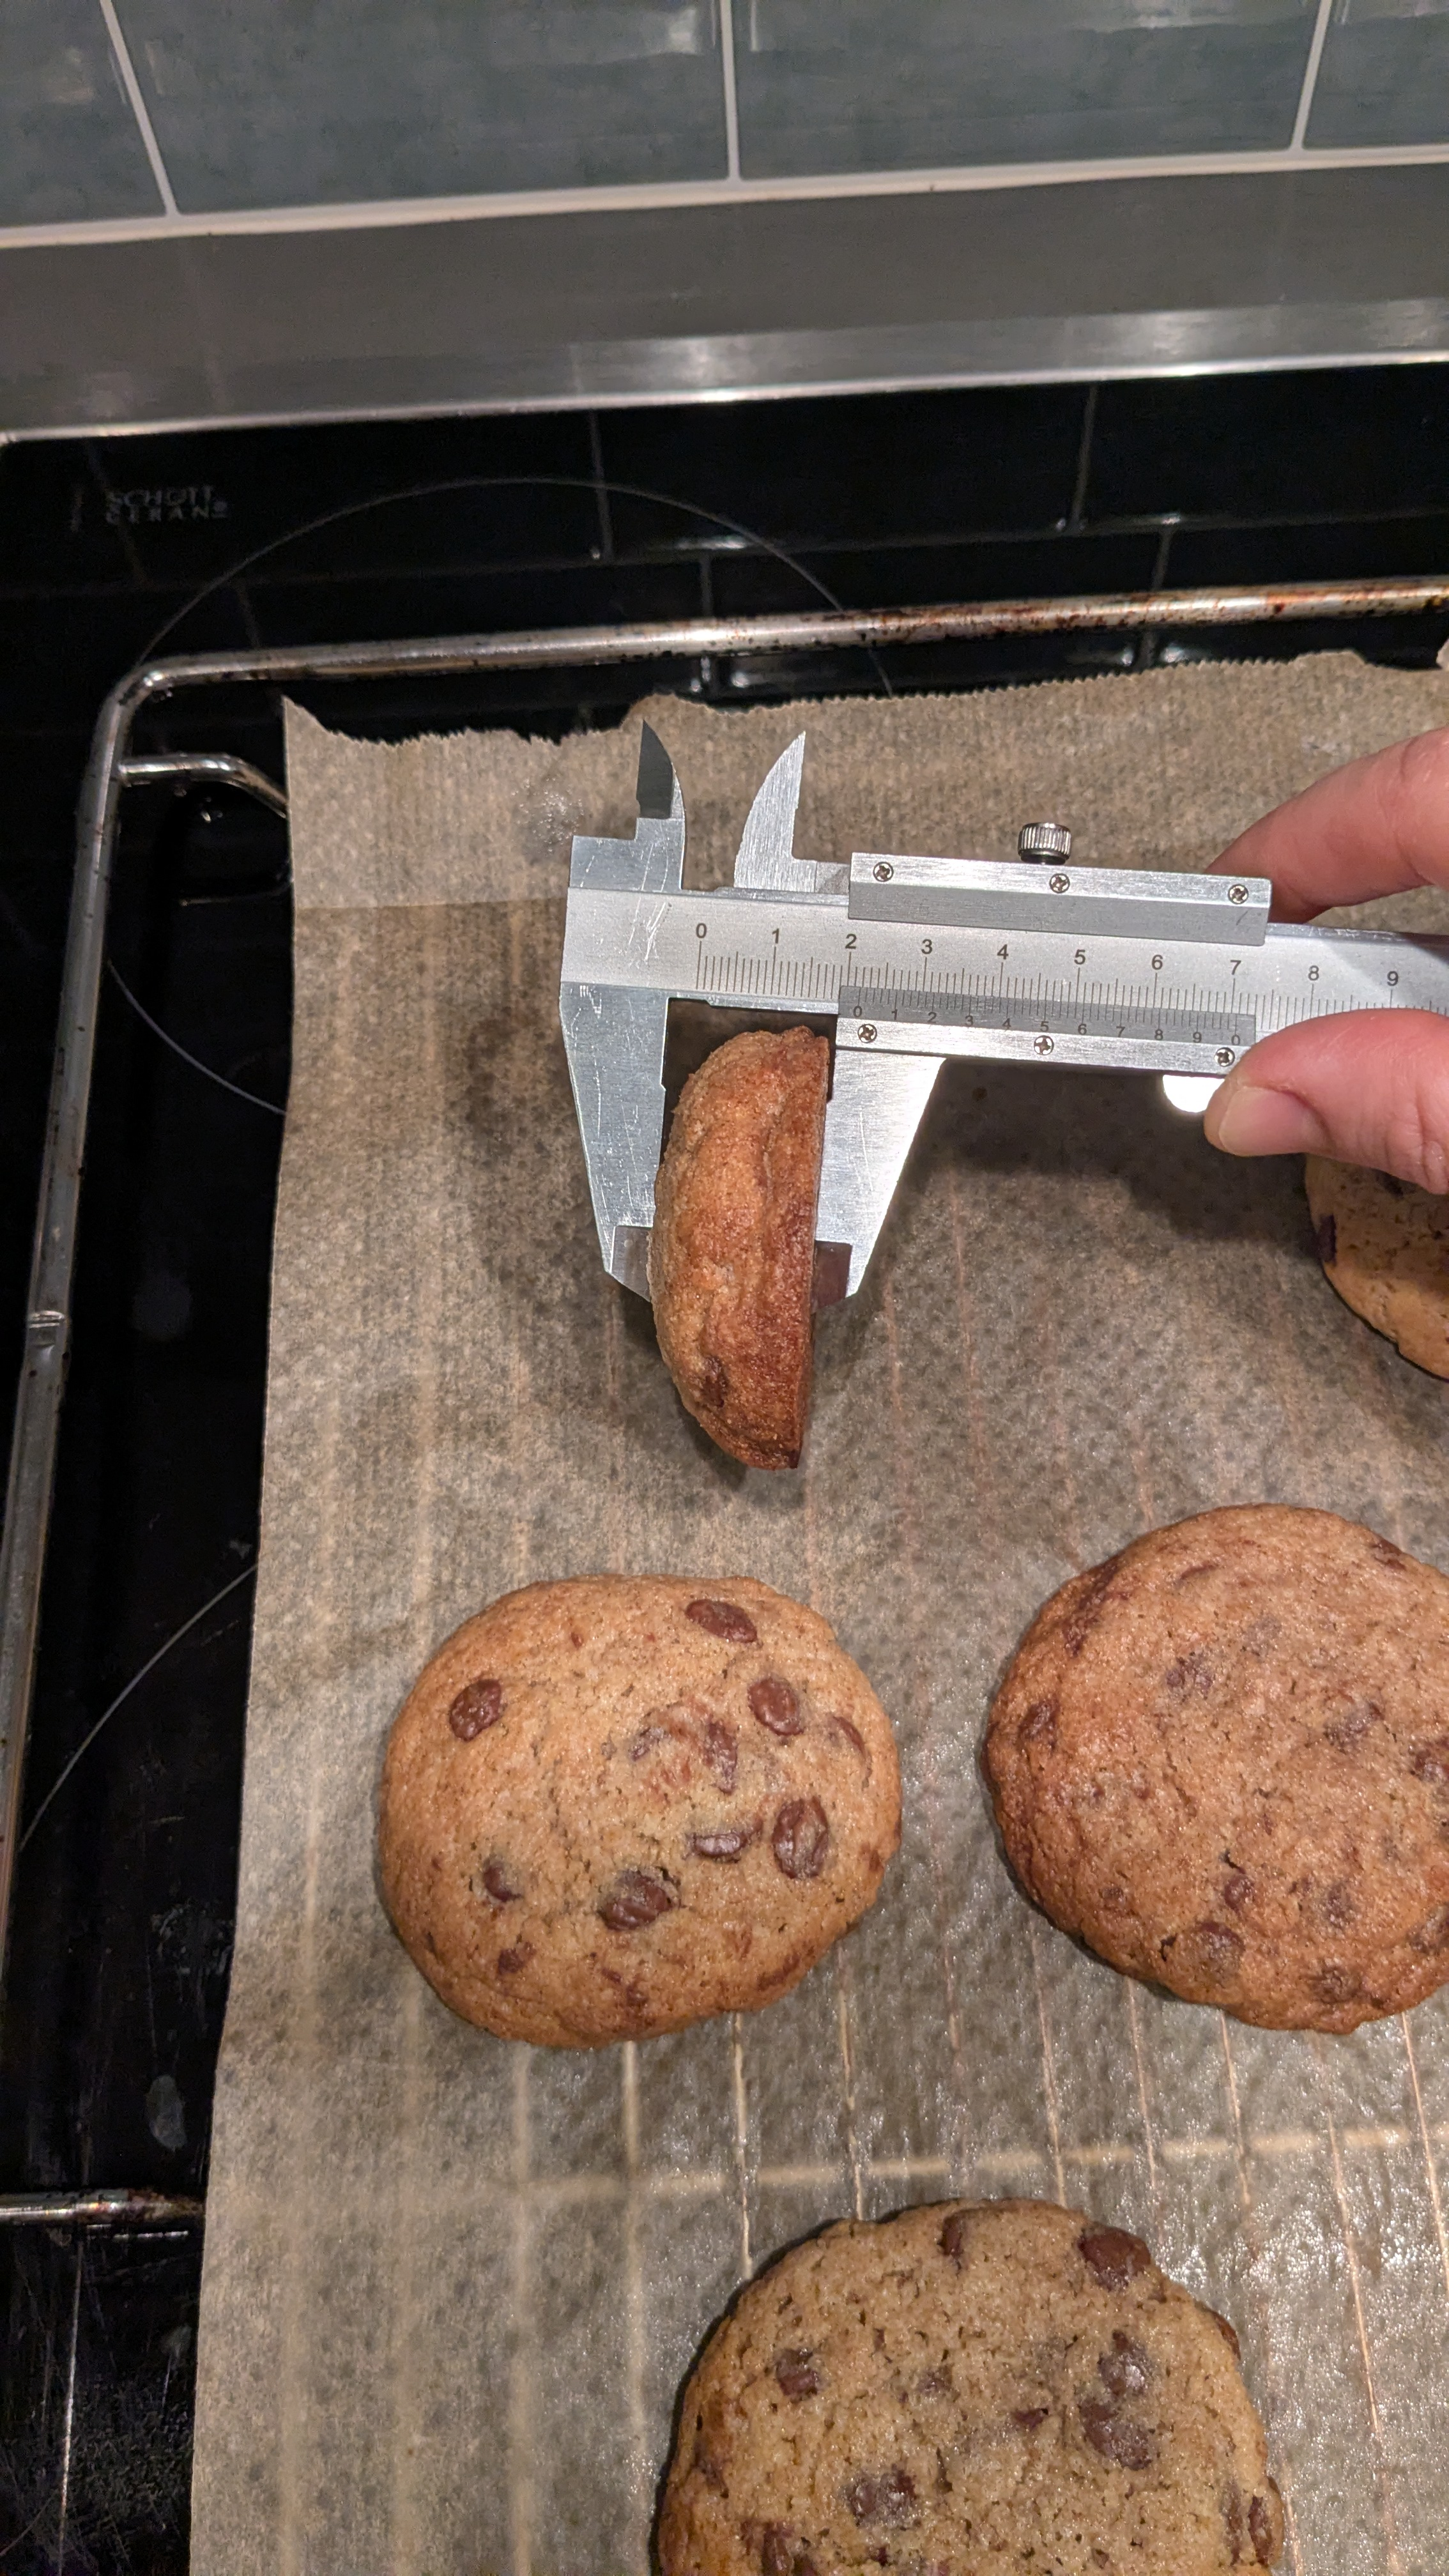
\includegraphics[width=0.5\linewidth]{figures/messung_hoehe.jpg}
    \caption{Messung der Höhe}
    \label{fig:messung_h}
\end{figure}

\chapter{Versuchsplan} \label{ch:appendix_versuch}
\vspace{-1.0\baselineskip}
\begin{table}
\centering
\caption{Versuchsplan}
\label{table:versuchsplan}
\begin{tabular}{|r|r|r|r|r|r|r|}
\hline
StdRfolge & DlaufRfolg & ZtrlPunkt & Bl"ocke & Butter\_g & Zucker\_g & Vollkornmehl\_\% \\
\hline
6  & 1  & 1 & 1 & 250 & 160 & 1  \\
1  & 2  & 1 & 1 & 120 & 160 & -1 \\
4  & 3  & 1 & 1 & 250 & 280 & -1 \\
10 & 4  & 0 & 1 & 185 & 220 & 0  \\
8  & 5  & 1 & 1 & 250 & 280 & 1  \\
7  & 6  & 1 & 1 & 120 & 280 & 1  \\
2  & 7  & 1 & 1 & 250 & 160 & -1 \\
9  & 8  & 0 & 1 & 185 & 220 & 0  \\
5  & 9  & 1 & 1 & 120 & 160 & 1  \\
3  & 10 & 1 & 1 & 120 & 280 & -1 \\
19 & 11 & 0 & 2 & 185 & 220 & 0  \\
15 & 12 & 1 & 2 & 120 & 160 & 1  \\
13 & 13 & 1 & 2 & 120 & 280 & -1 \\
20 & 14 & 0 & 2 & 185 & 220 & 0  \\
16 & 15 & 1 & 2 & 250 & 160 & 1  \\
11 & 16 & 1 & 2 & 120 & 160 & -1 \\
14 & 17 & 1 & 2 & 250 & 280 & -1 \\
18 & 18 & 1 & 2 & 250 & 280 & 1  \\
17 & 19 & 1 & 2 & 120 & 280 & 1  \\
12 & 20 & 1 & 2 & 250 & 160 & -1 \\
28 & 21 & 1 & 3 & 250 & 280 & 1  \\
27 & 22 & 1 & 3 & 120 & 280 & 1  \\
22 & 23 & 1 & 3 & 250 & 160 & -1 \\
30 & 24 & 0 & 3 & 185 & 220 & 0  \\
29 & 25 & 0 & 3 & 185 & 220 & 0  \\
25 & 26 & 1 & 3 & 120 & 160 & 1  \\
23 & 27 & 1 & 3 & 120 & 280 & -1 \\
26 & 28 & 1 & 3 & 250 & 160 & 1  \\
21 & 29 & 1 & 3 & 120 & 160 & -1 \\
24 & 30 & 1 & 3 & 250 & 280 & -1 \\
\hline
\end{tabular}
\end{table}


\chapter{Ergebnisse} \label{ch:appendix_ergebnisse}
\vspace{-1.0\baselineskip}
\begin{table}[H]
\centering
\caption{Versuchsergebnisse: Durchmesser und Höhe in mm}
\label{tab:ergebnisse}
\begin{tabular}{|r|r|r|r|r|}
\hline
DlaufRfolg & Durchmesser\_1 & Durchmesser\_2 & Höhe & Durchsch\_Durchmesser \\
\hline
1 & 59 & 61 & 23 & 60 \\
2 & 61 & 64 & 21 & 62,5 \\
3 & 89 & 83 & 8 & 86 \\
4 & 66 & 73 & 16 & 69,5 \\
5 & 76 & 76 & 14 & 76 \\
6 & 67 & 67 & 16 & 67 \\
7 & 73 & 69 & 19 & 71 \\
8 & 70 & 72 & 15 & 71 \\
9 & 59 & 56 & 22 & 57,5 \\
10 & 79 & 78 & 13 & 78,5 \\
\hline
11 & 69 & 69 & 16 & 69 \\
12 & 58 & 57 & 22 & 57,5 \\
13 & 80 & 76 & 11 & 78 \\
14 & 69 & 70 & 16 & 69,5 \\
15 & 64 & 64 & 18 & 64 \\
16 & 66 & 64 & 20 & 65 \\
17 & 90 & 88 & 9 & 89 \\
18 & 77 & 83 & 13 & 80 \\
19 & 69 & 69 & 17 & 69 \\
20 & 75 & 75 & 17 & 75 \\
\hline
21 & 77 & 78 & 15 & 77,5 \\
22 & 70 & 70 & 16 & 70 \\
23 & 75 & 73 & 17 & 74 \\
24 & 73 & 70 & 17 & 71,5 \\
25 & 74 & 69 & 15 & 71,5 \\
26 & 61 & 59 & 22 & 60 \\
27 & 80 & 80 & 13 & 80 \\
28 & 67 & 67 & 21 & 67 \\
29 & 65 & 68 & 19 & 66,5 \\
30 & 94 & 89 & 9 & 91,5 \\
\hline
\end{tabular}
\end{table}


\chapter{Dokumentation der Durchführung} \label{ch:appendix_durchf}
\vspace{-1.0\baselineskip}

\begin{figure}[H]
\centering
\begin{subfigure}{0.49\textwidth}
    \centering
    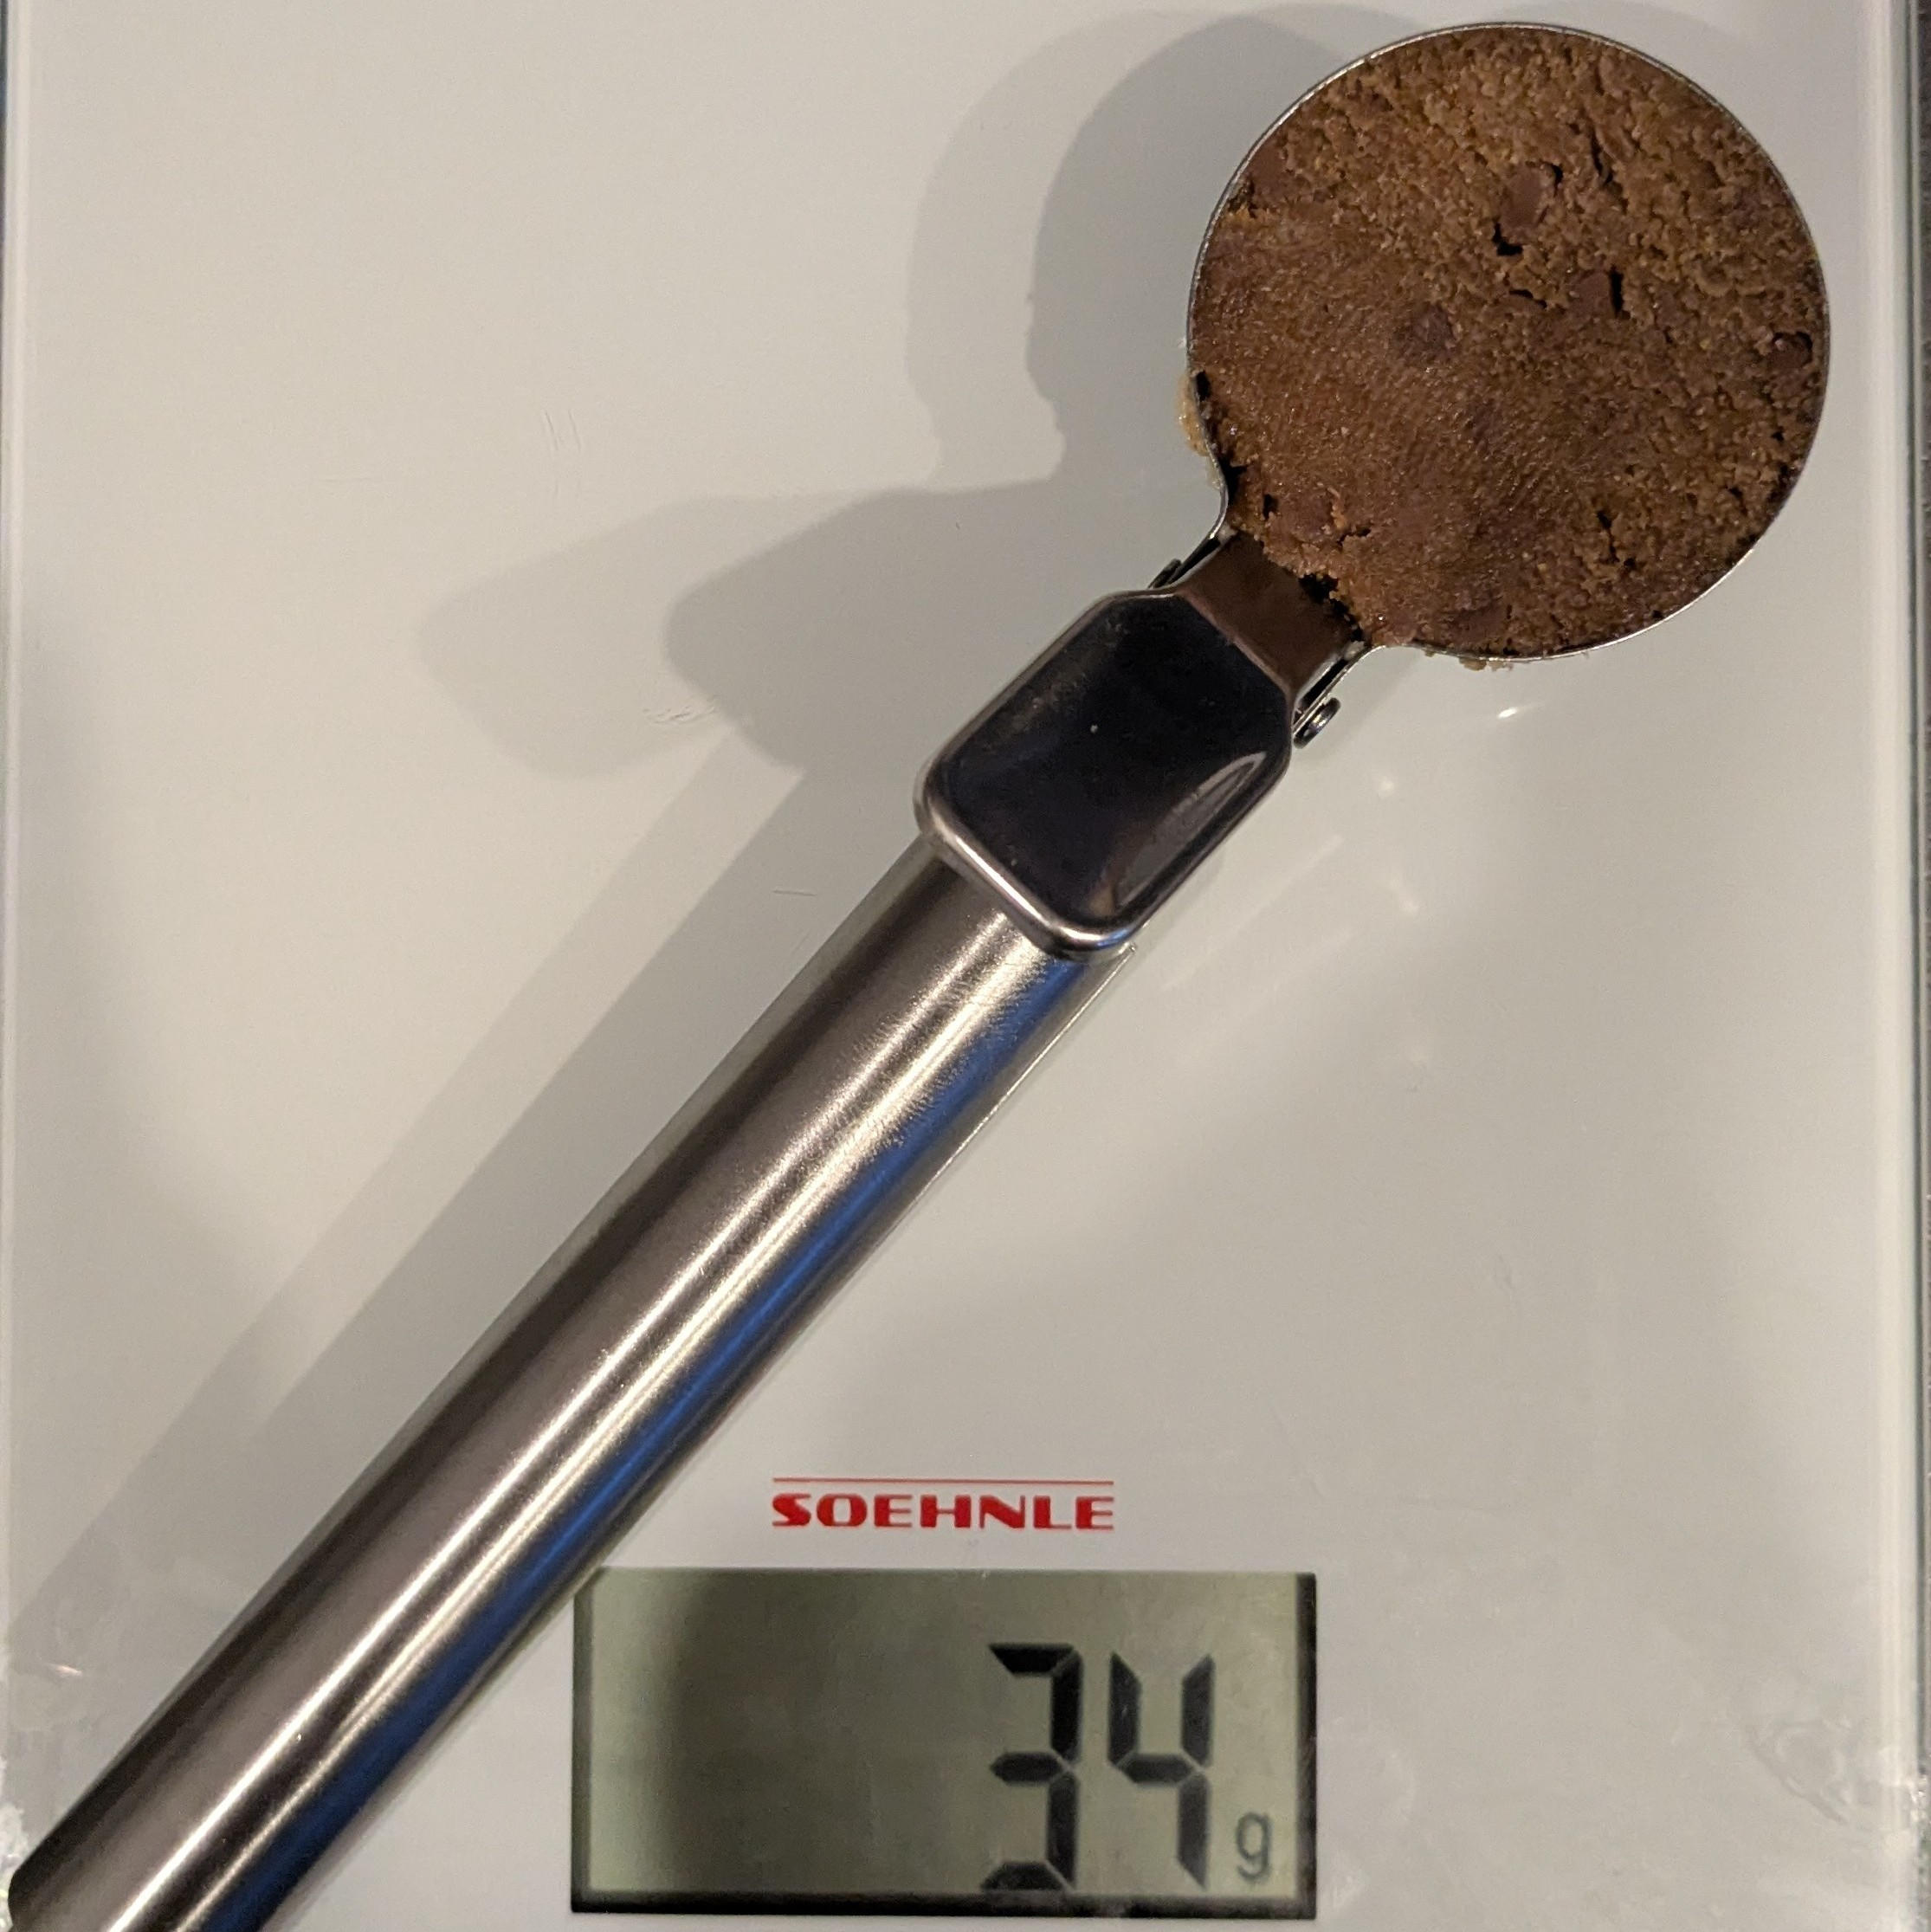
\includegraphics[width=\textwidth]{figures/portionierung_gewicht.jpg}
    \caption{Portionierung eines Cookies mit Gewichtsmessung}
    \label{fig:portionierung}
\end{subfigure}\hfill
\begin{subfigure}{0.49\textwidth}
    \centering
    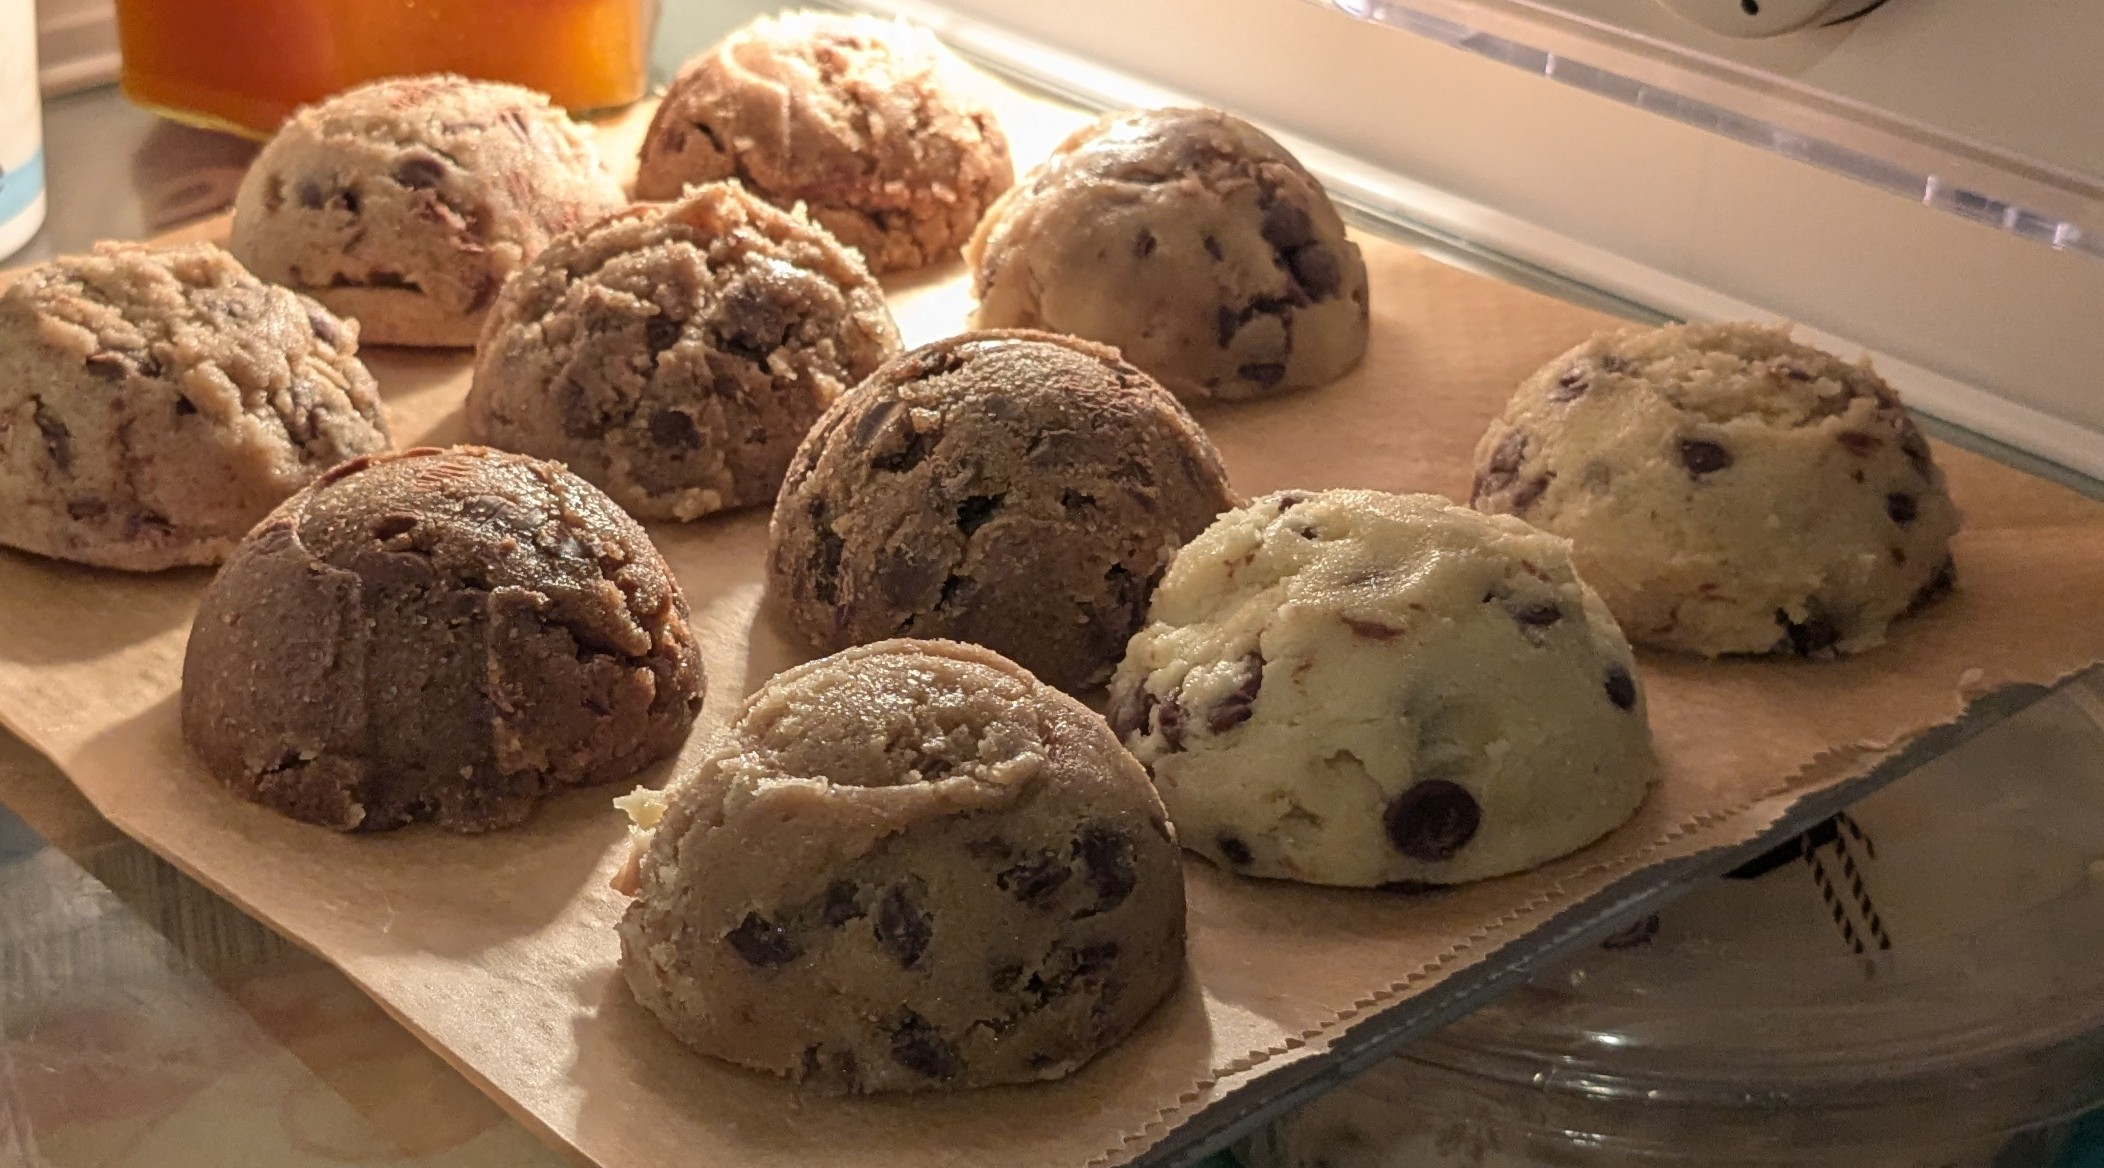
\includegraphics[width=\textwidth]{figures/portionen_vorbereitung_klein.jpg}
    \caption{Kühlung der Cookies während des Portionierens}
    \label{fig:kühlung}
\end{subfigure}
\caption{Portionierung und Vorbereitung}
\label{fig:portionierung}
\end{figure}

\begin{figure}[H]
\centering
\begin{subfigure}{0.49\textwidth}
    \centering
    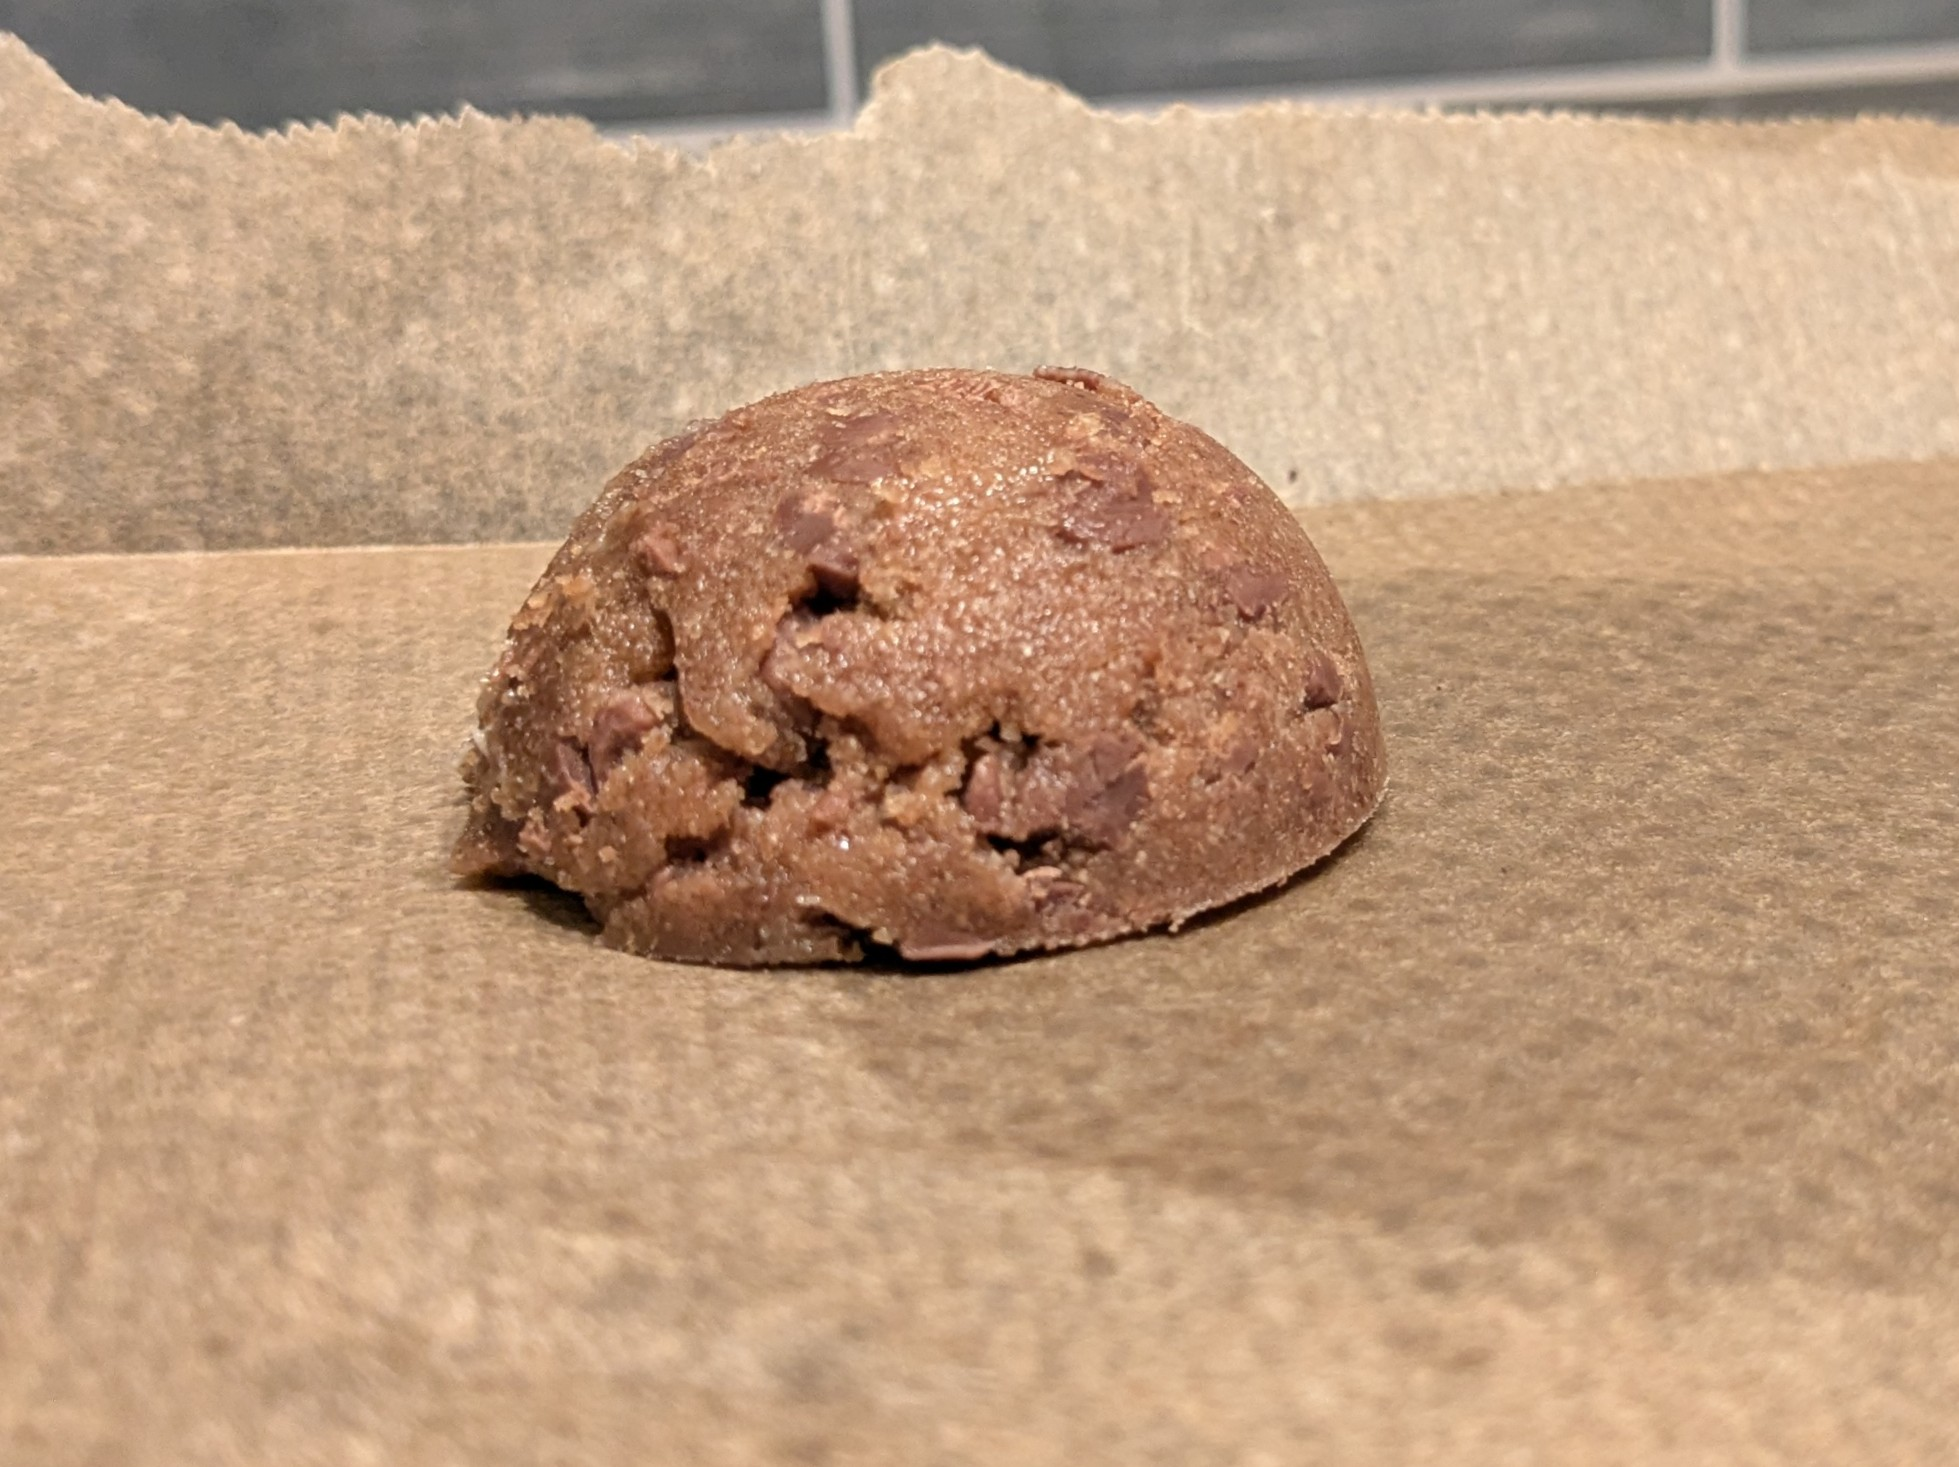
\includegraphics[width=\textwidth]{figures/portion_seitlich.jpg}
    \caption{Seitliche Sicht}
    \label{fig:portion_seitlich}
\end{subfigure}\hfill
\begin{subfigure}{0.49\textwidth}
    \centering
    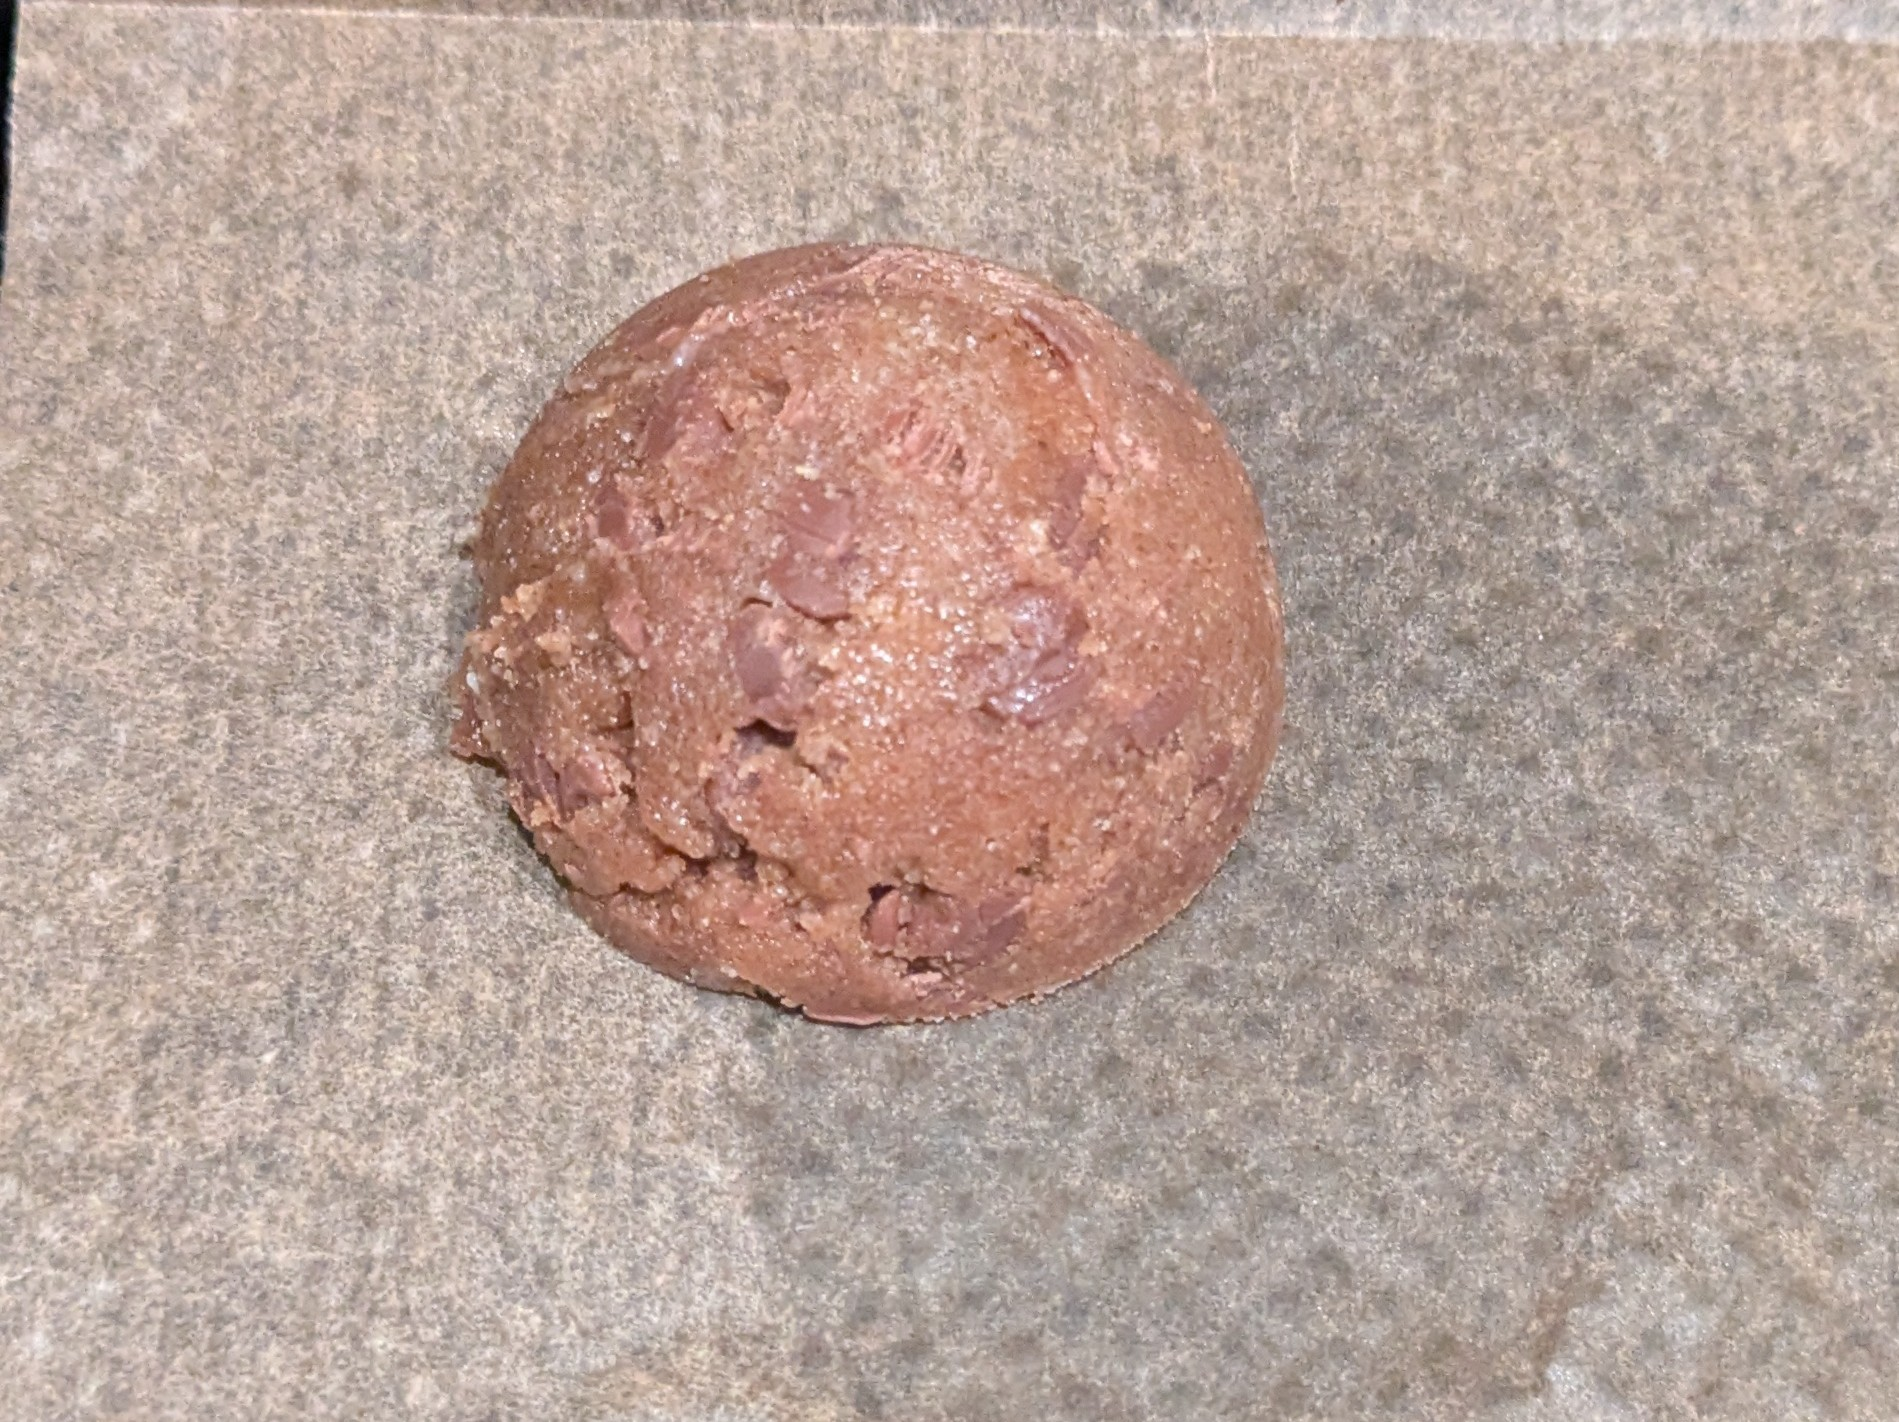
\includegraphics[width=\textwidth]{figures/portion_oben.jpg}
    \caption{Draufsicht}
    \label{fig:portion_draufsicht}
\end{subfigure}
\caption{Ansicht einer Portion}
\label{fig:portion}
\end{figure}

\begin{figure}[H]
\centering
\begin{subfigure}{0.49\textwidth}
\centering
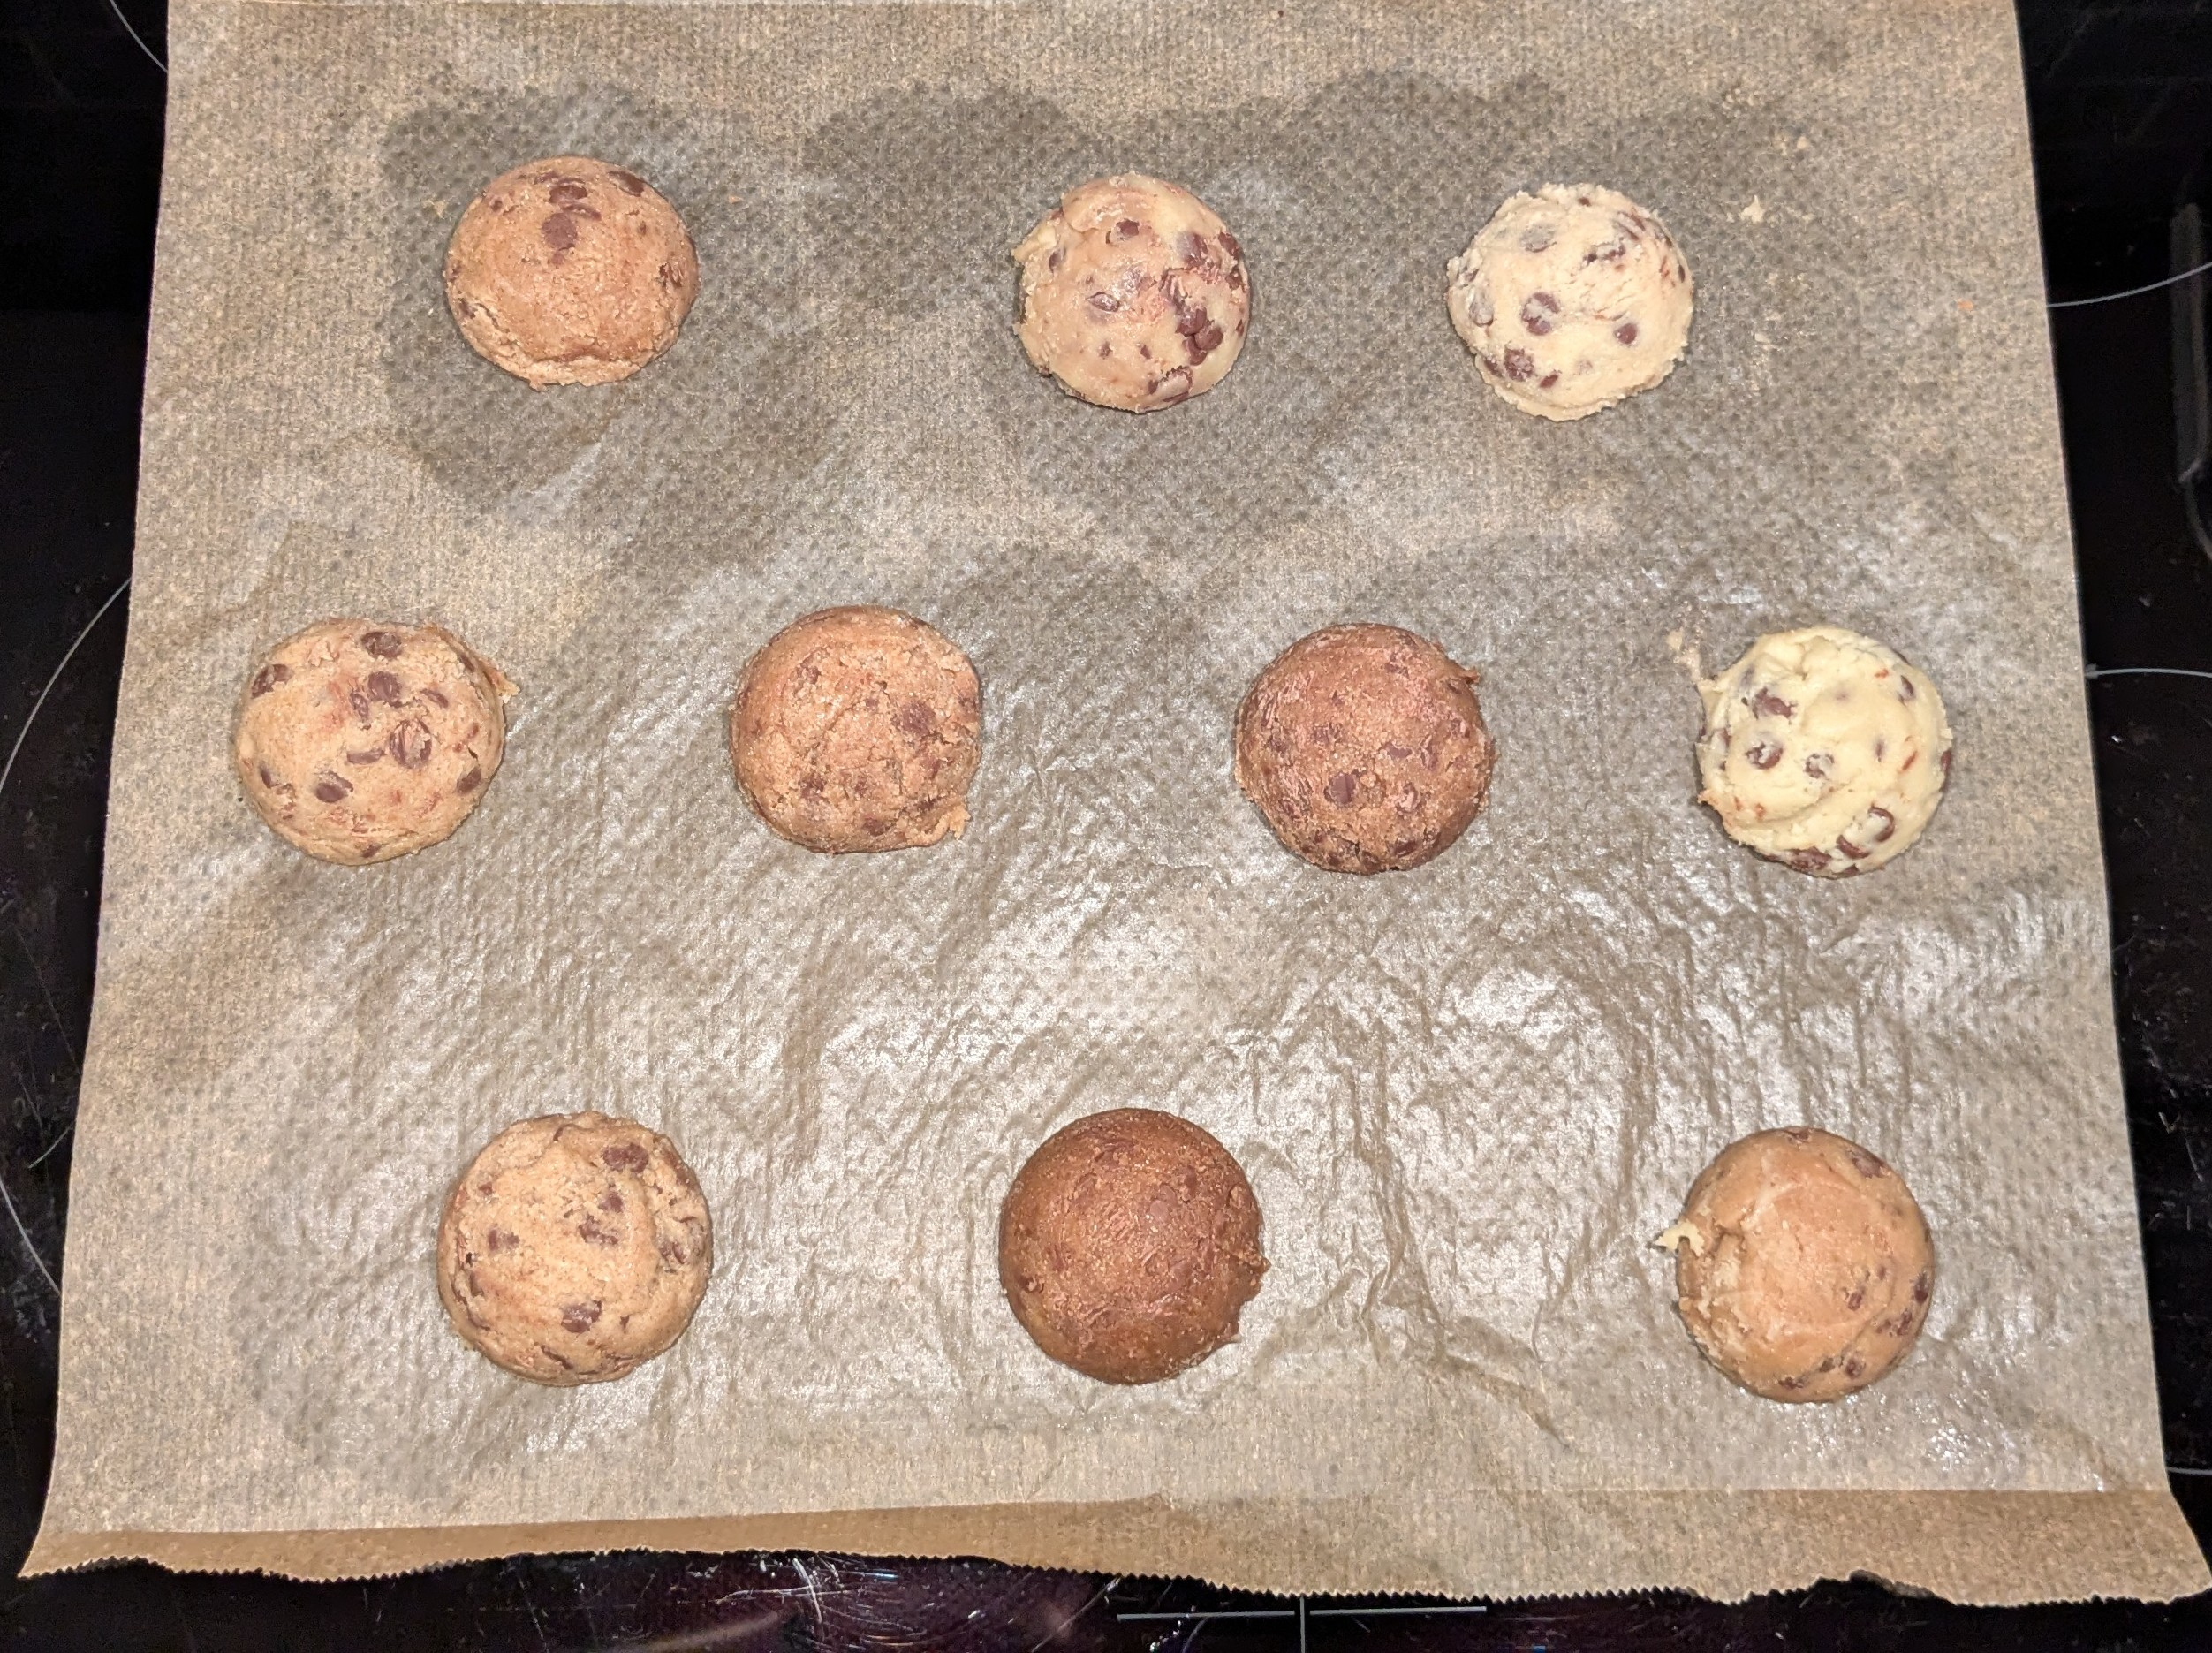
\includegraphics[width = \textwidth]{figures/block1_1_vorher.jpg}
\caption{Teigrohlinge vor dem Backen}
\label{fig:block1_1_vorher}
\end{subfigure}\hfill
\begin{subfigure}{0.49\textwidth}
\centering
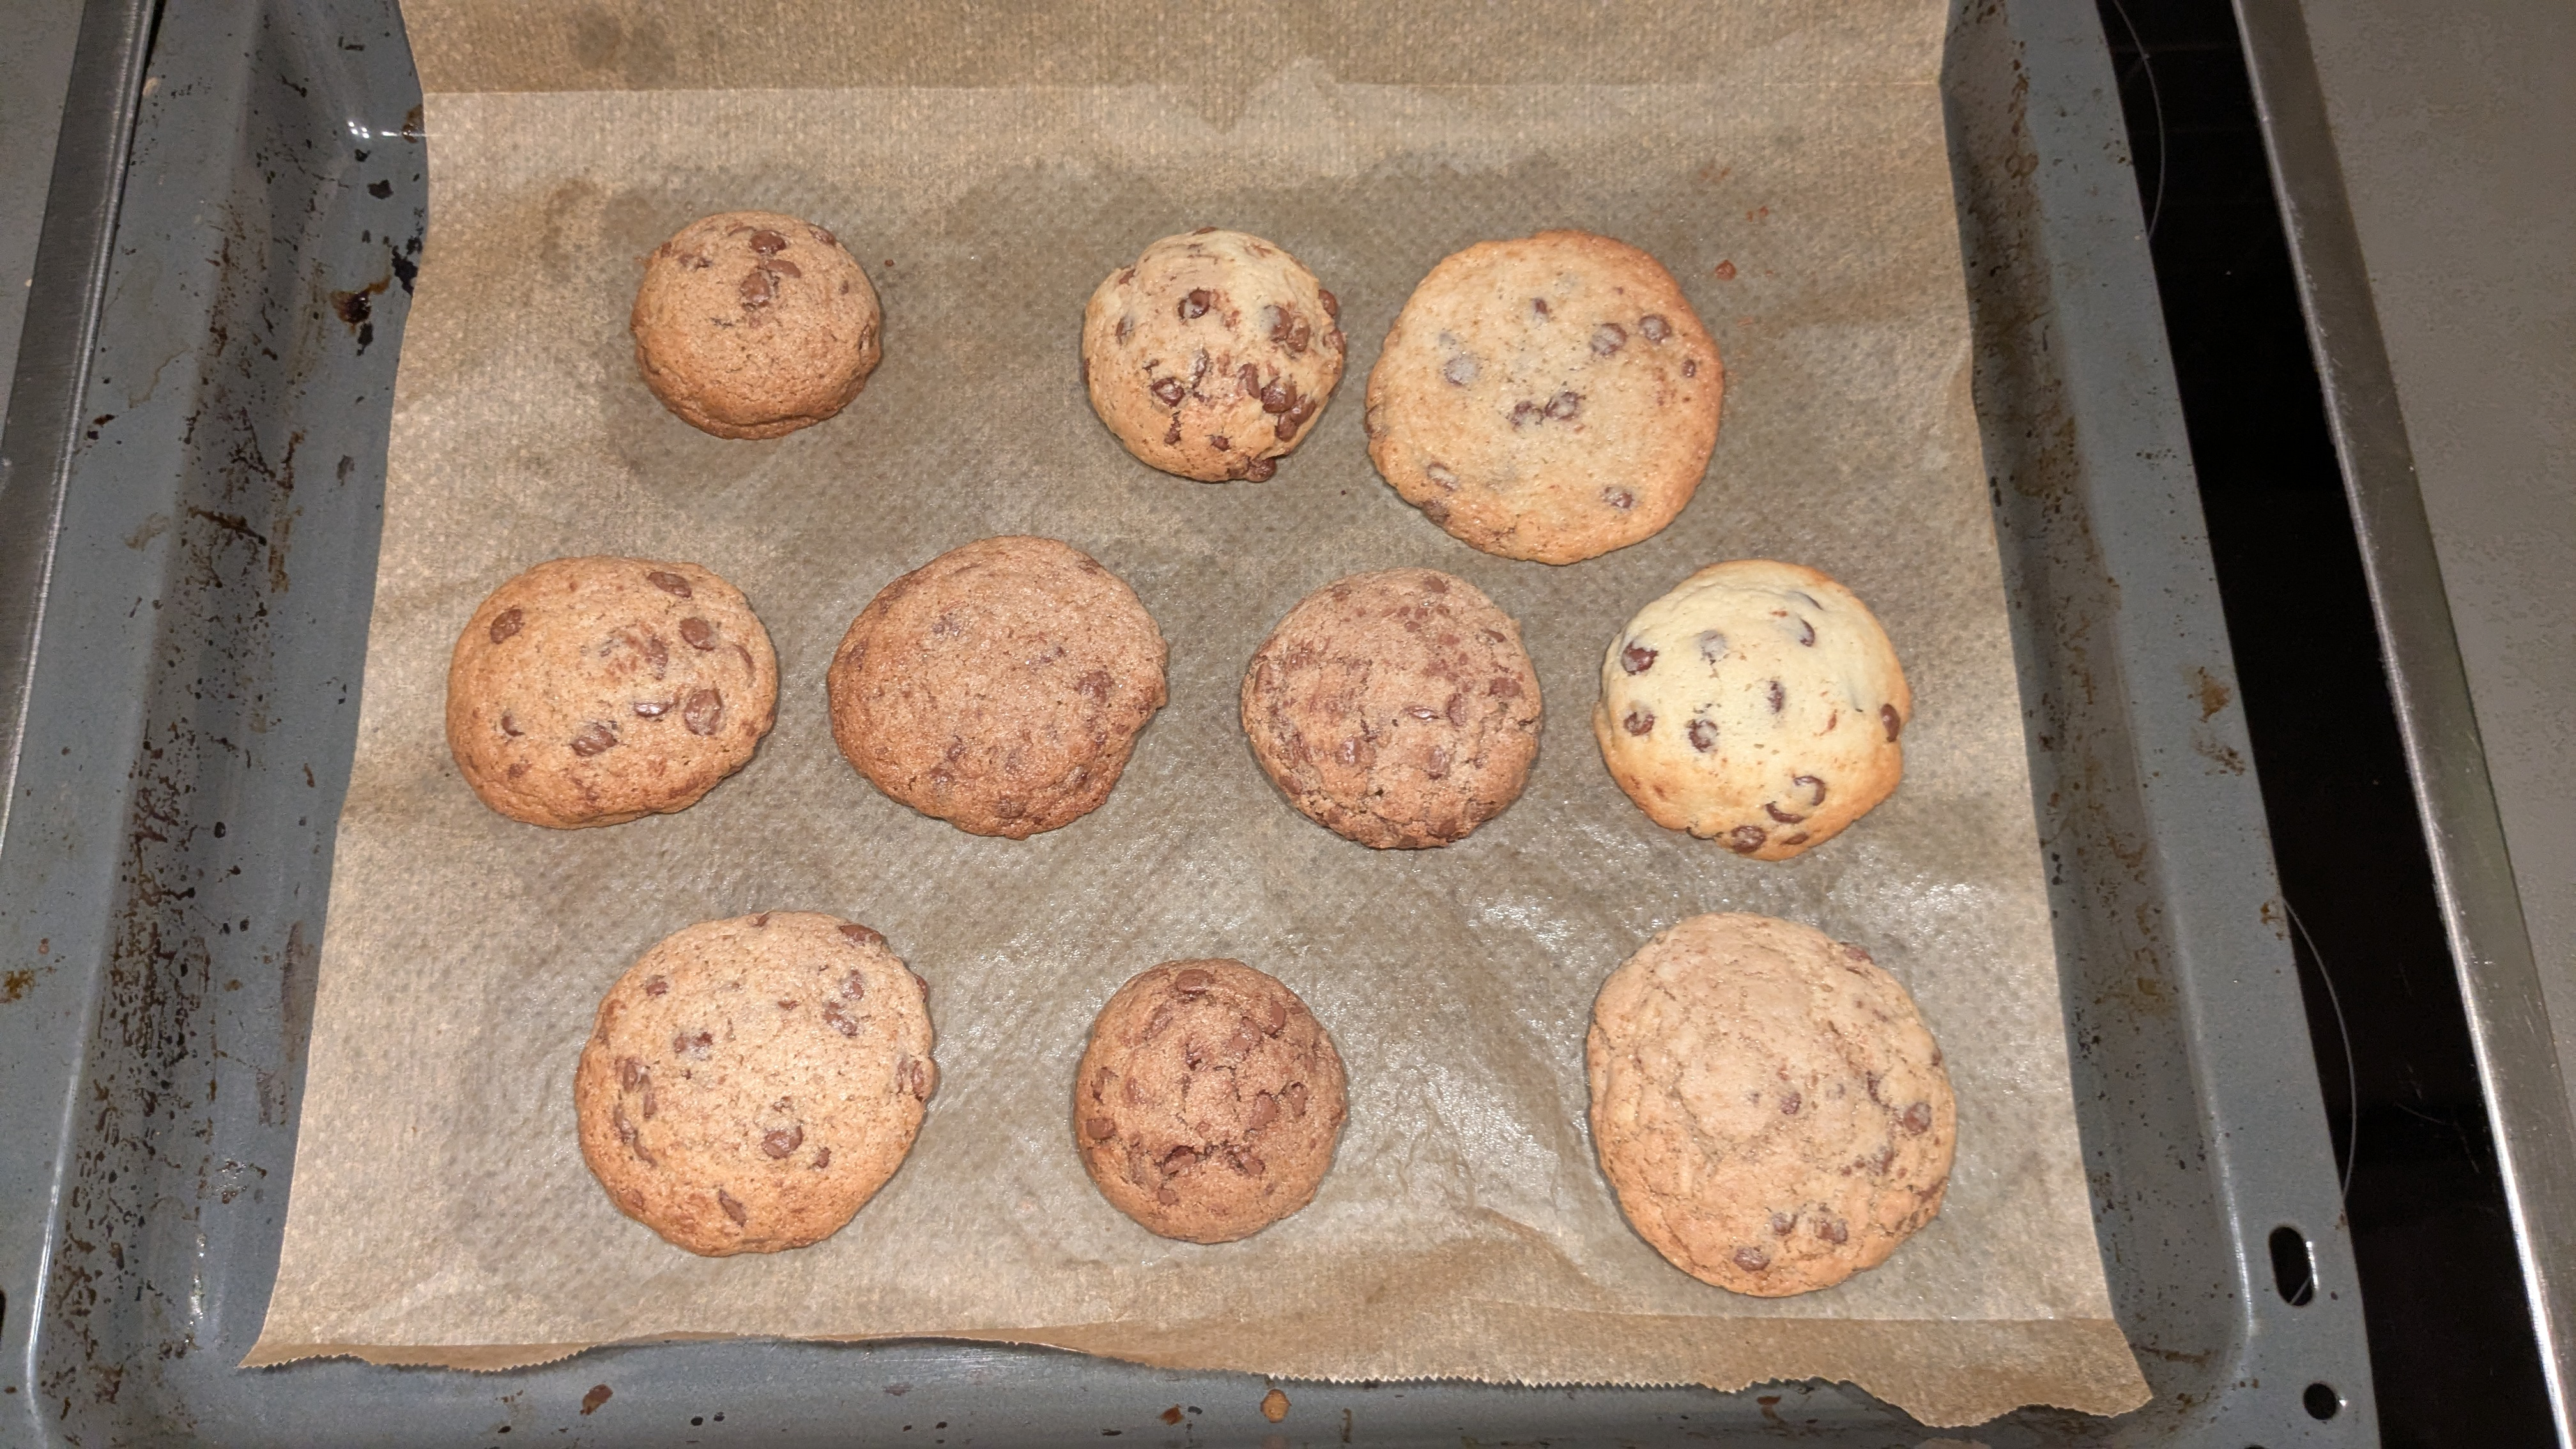
\includegraphics[width = \textwidth]{figures/block1_4_nacher.jpg}
\caption{Cookies nach dem Backvorgang}
\label{fig:block1_4_nacher}
\end{subfigure}
\caption{Backvorgang der ersten Replikation}
\label{fig:block_1}
\end{figure}

\begin{figure}[H]
\centering
\begin{subfigure}{0.49\textwidth}
\centering
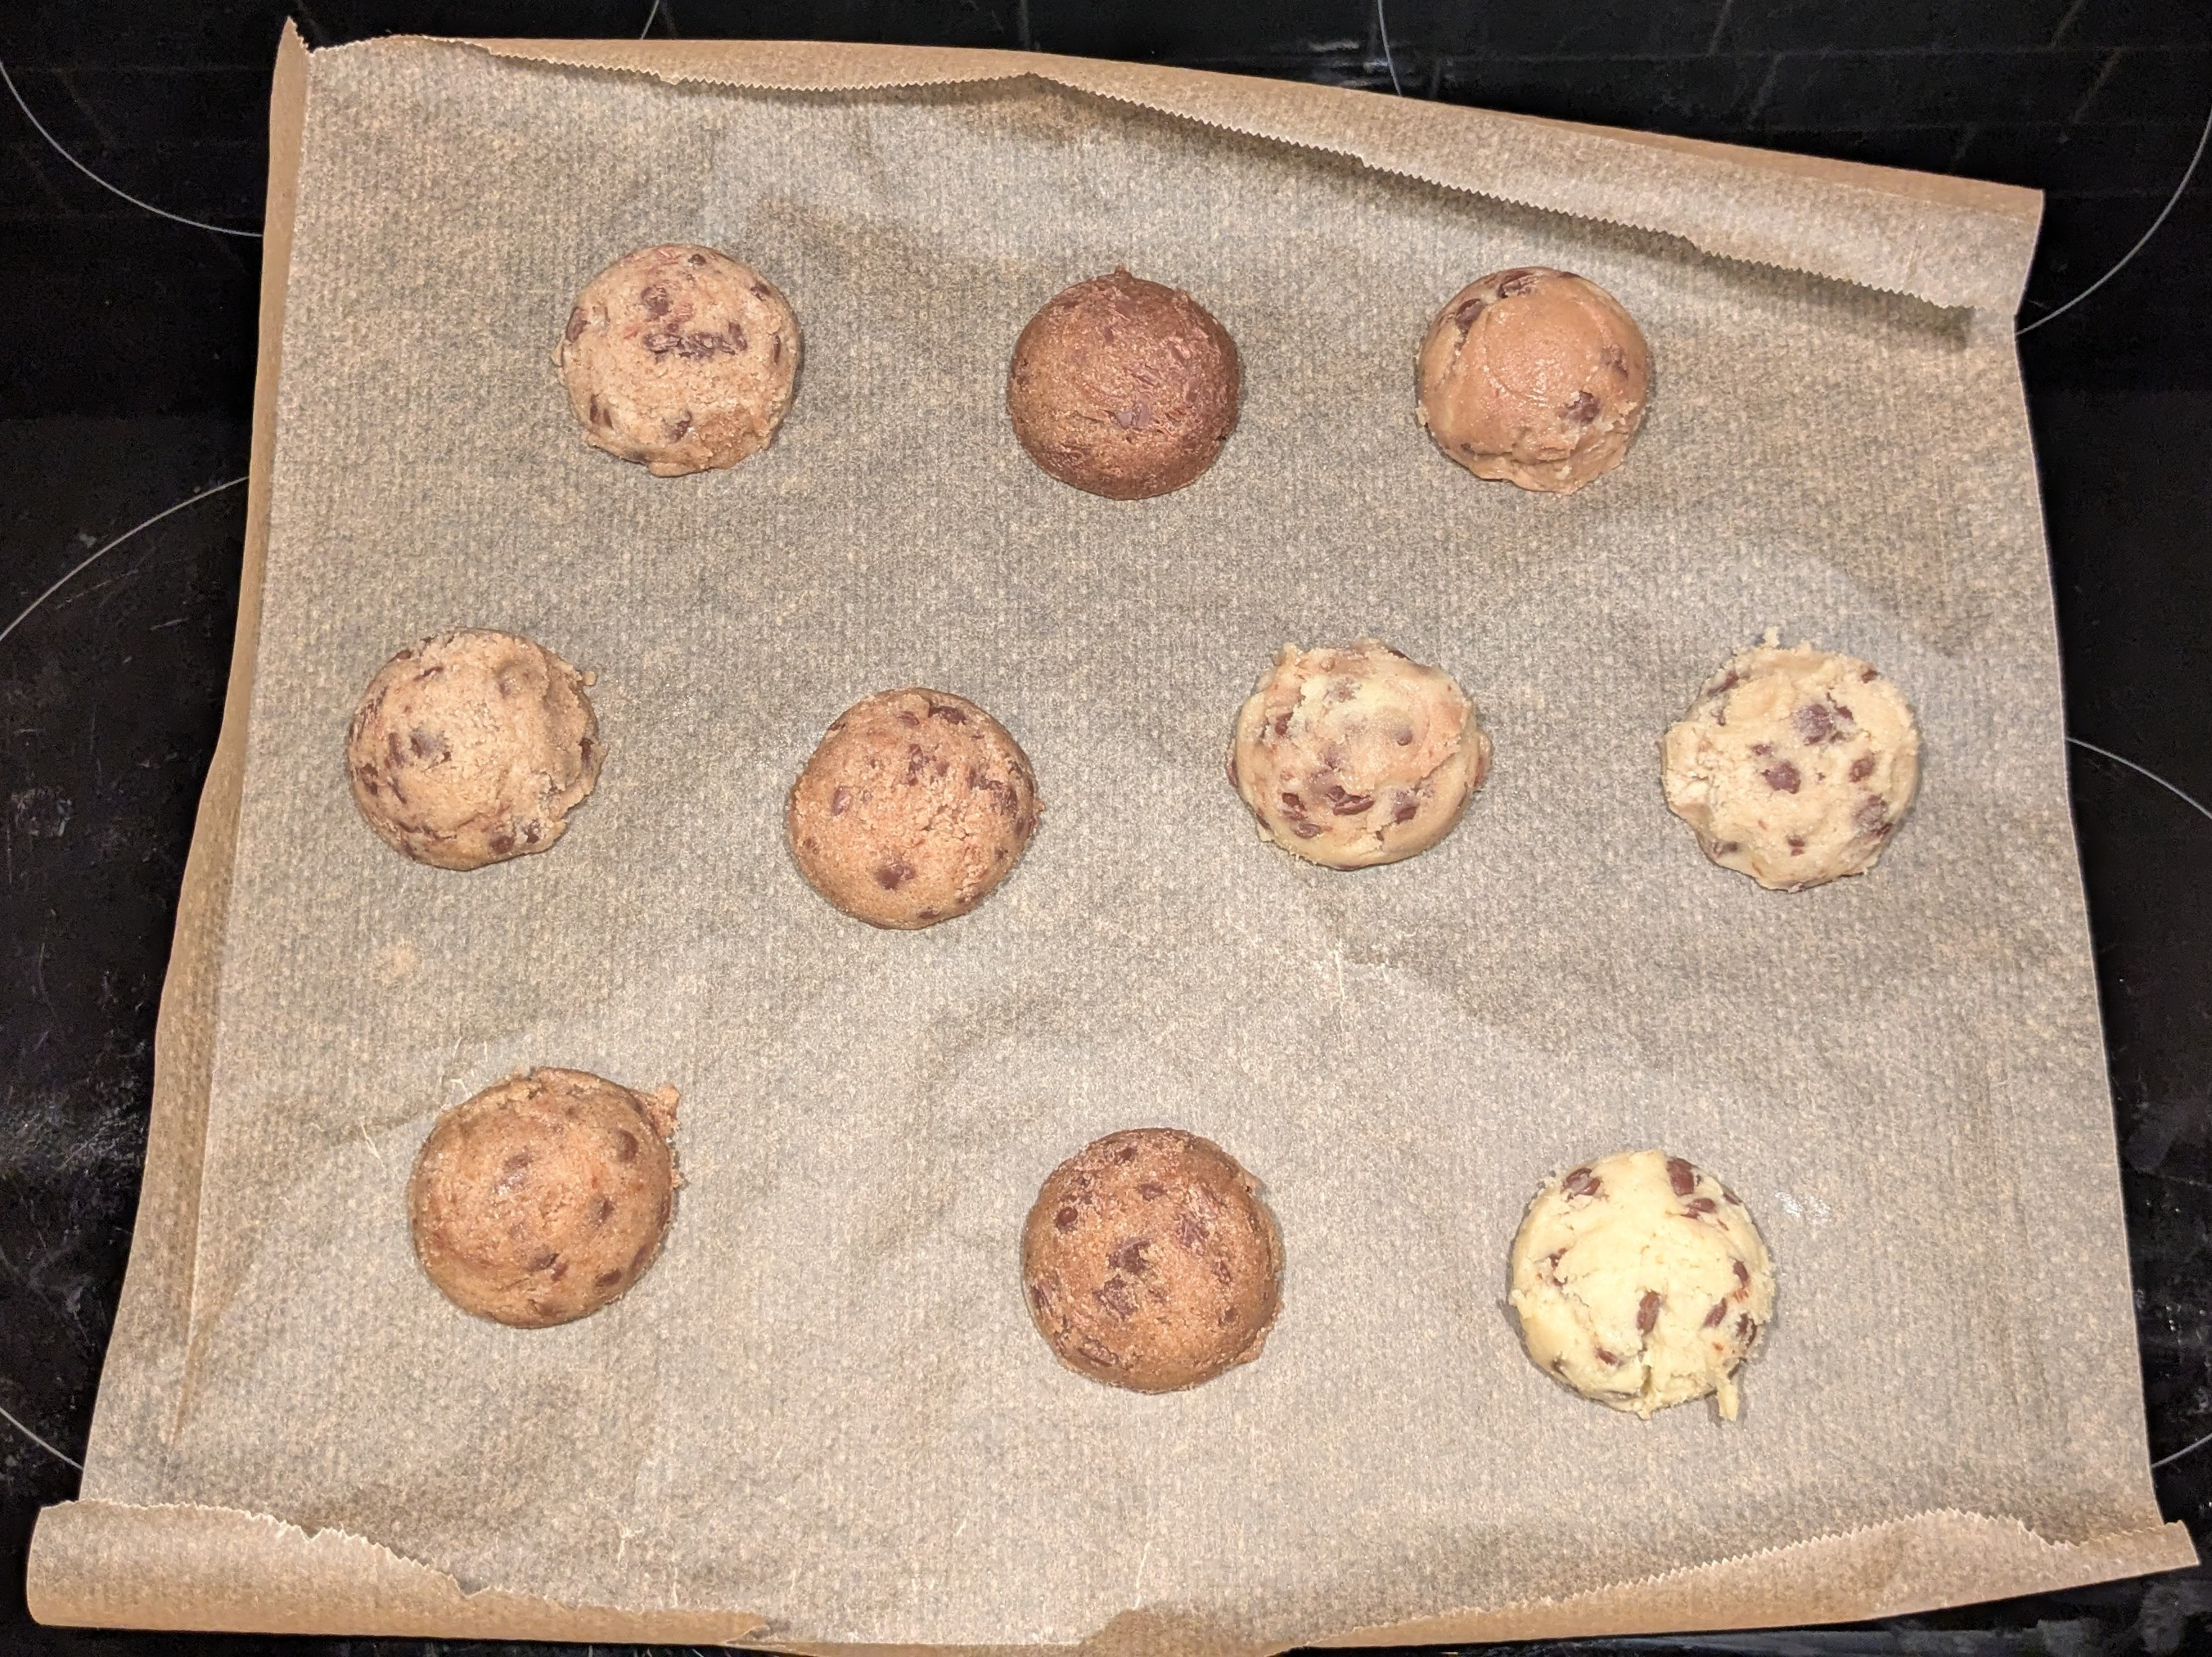
\includegraphics[width = \textwidth]{figures/block2_1_vorher.jpg}
\caption{Teigrohlinge vor dem Backen}
\label{fig:block2_1_vorher}
\end{subfigure}\hfill
\begin{subfigure}{0.49\textwidth}
\centering
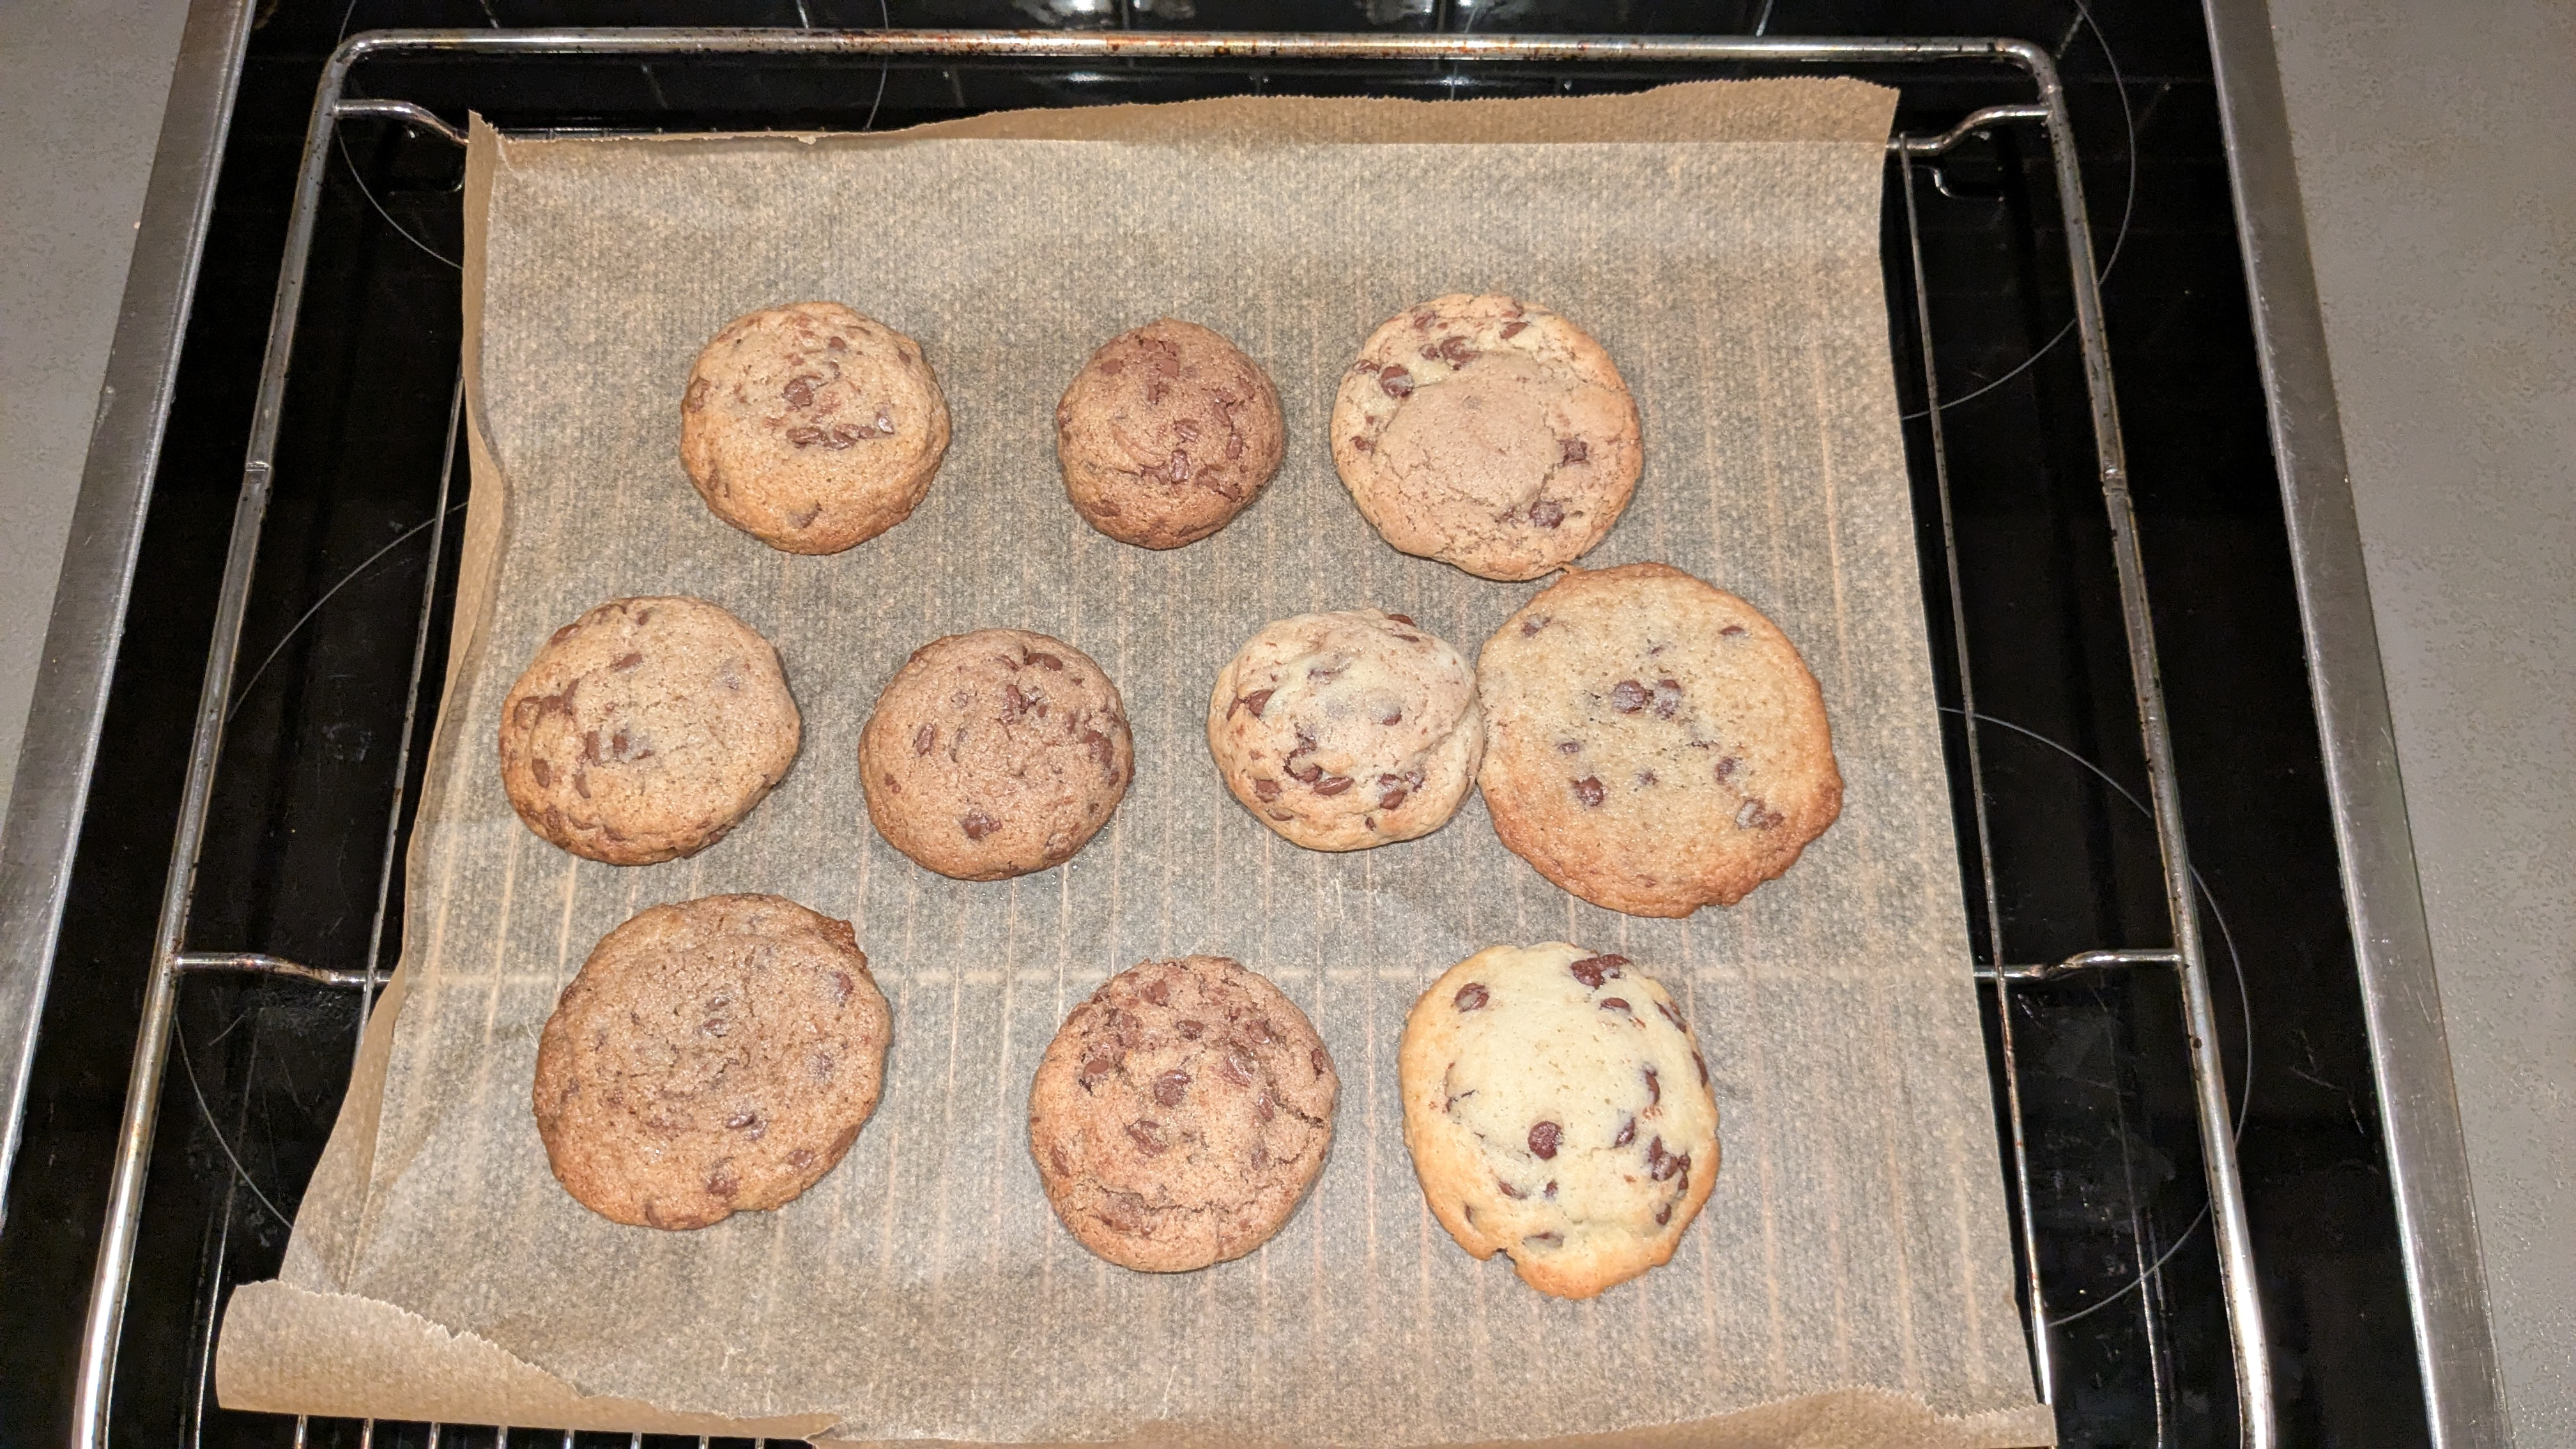
\includegraphics[width = \textwidth]{figures/block2_3_nachher.jpg}
\caption{Cookies nach dem Backvorgang}
\label{fig:block2_3_nacher}
\end{subfigure}

\caption{Backvorgang der zweiten Replikation}
\label{fig:block_2}
\end{figure}

\begin{figure}
\centering
\begin{subfigure}{0.49\textwidth}
\centering
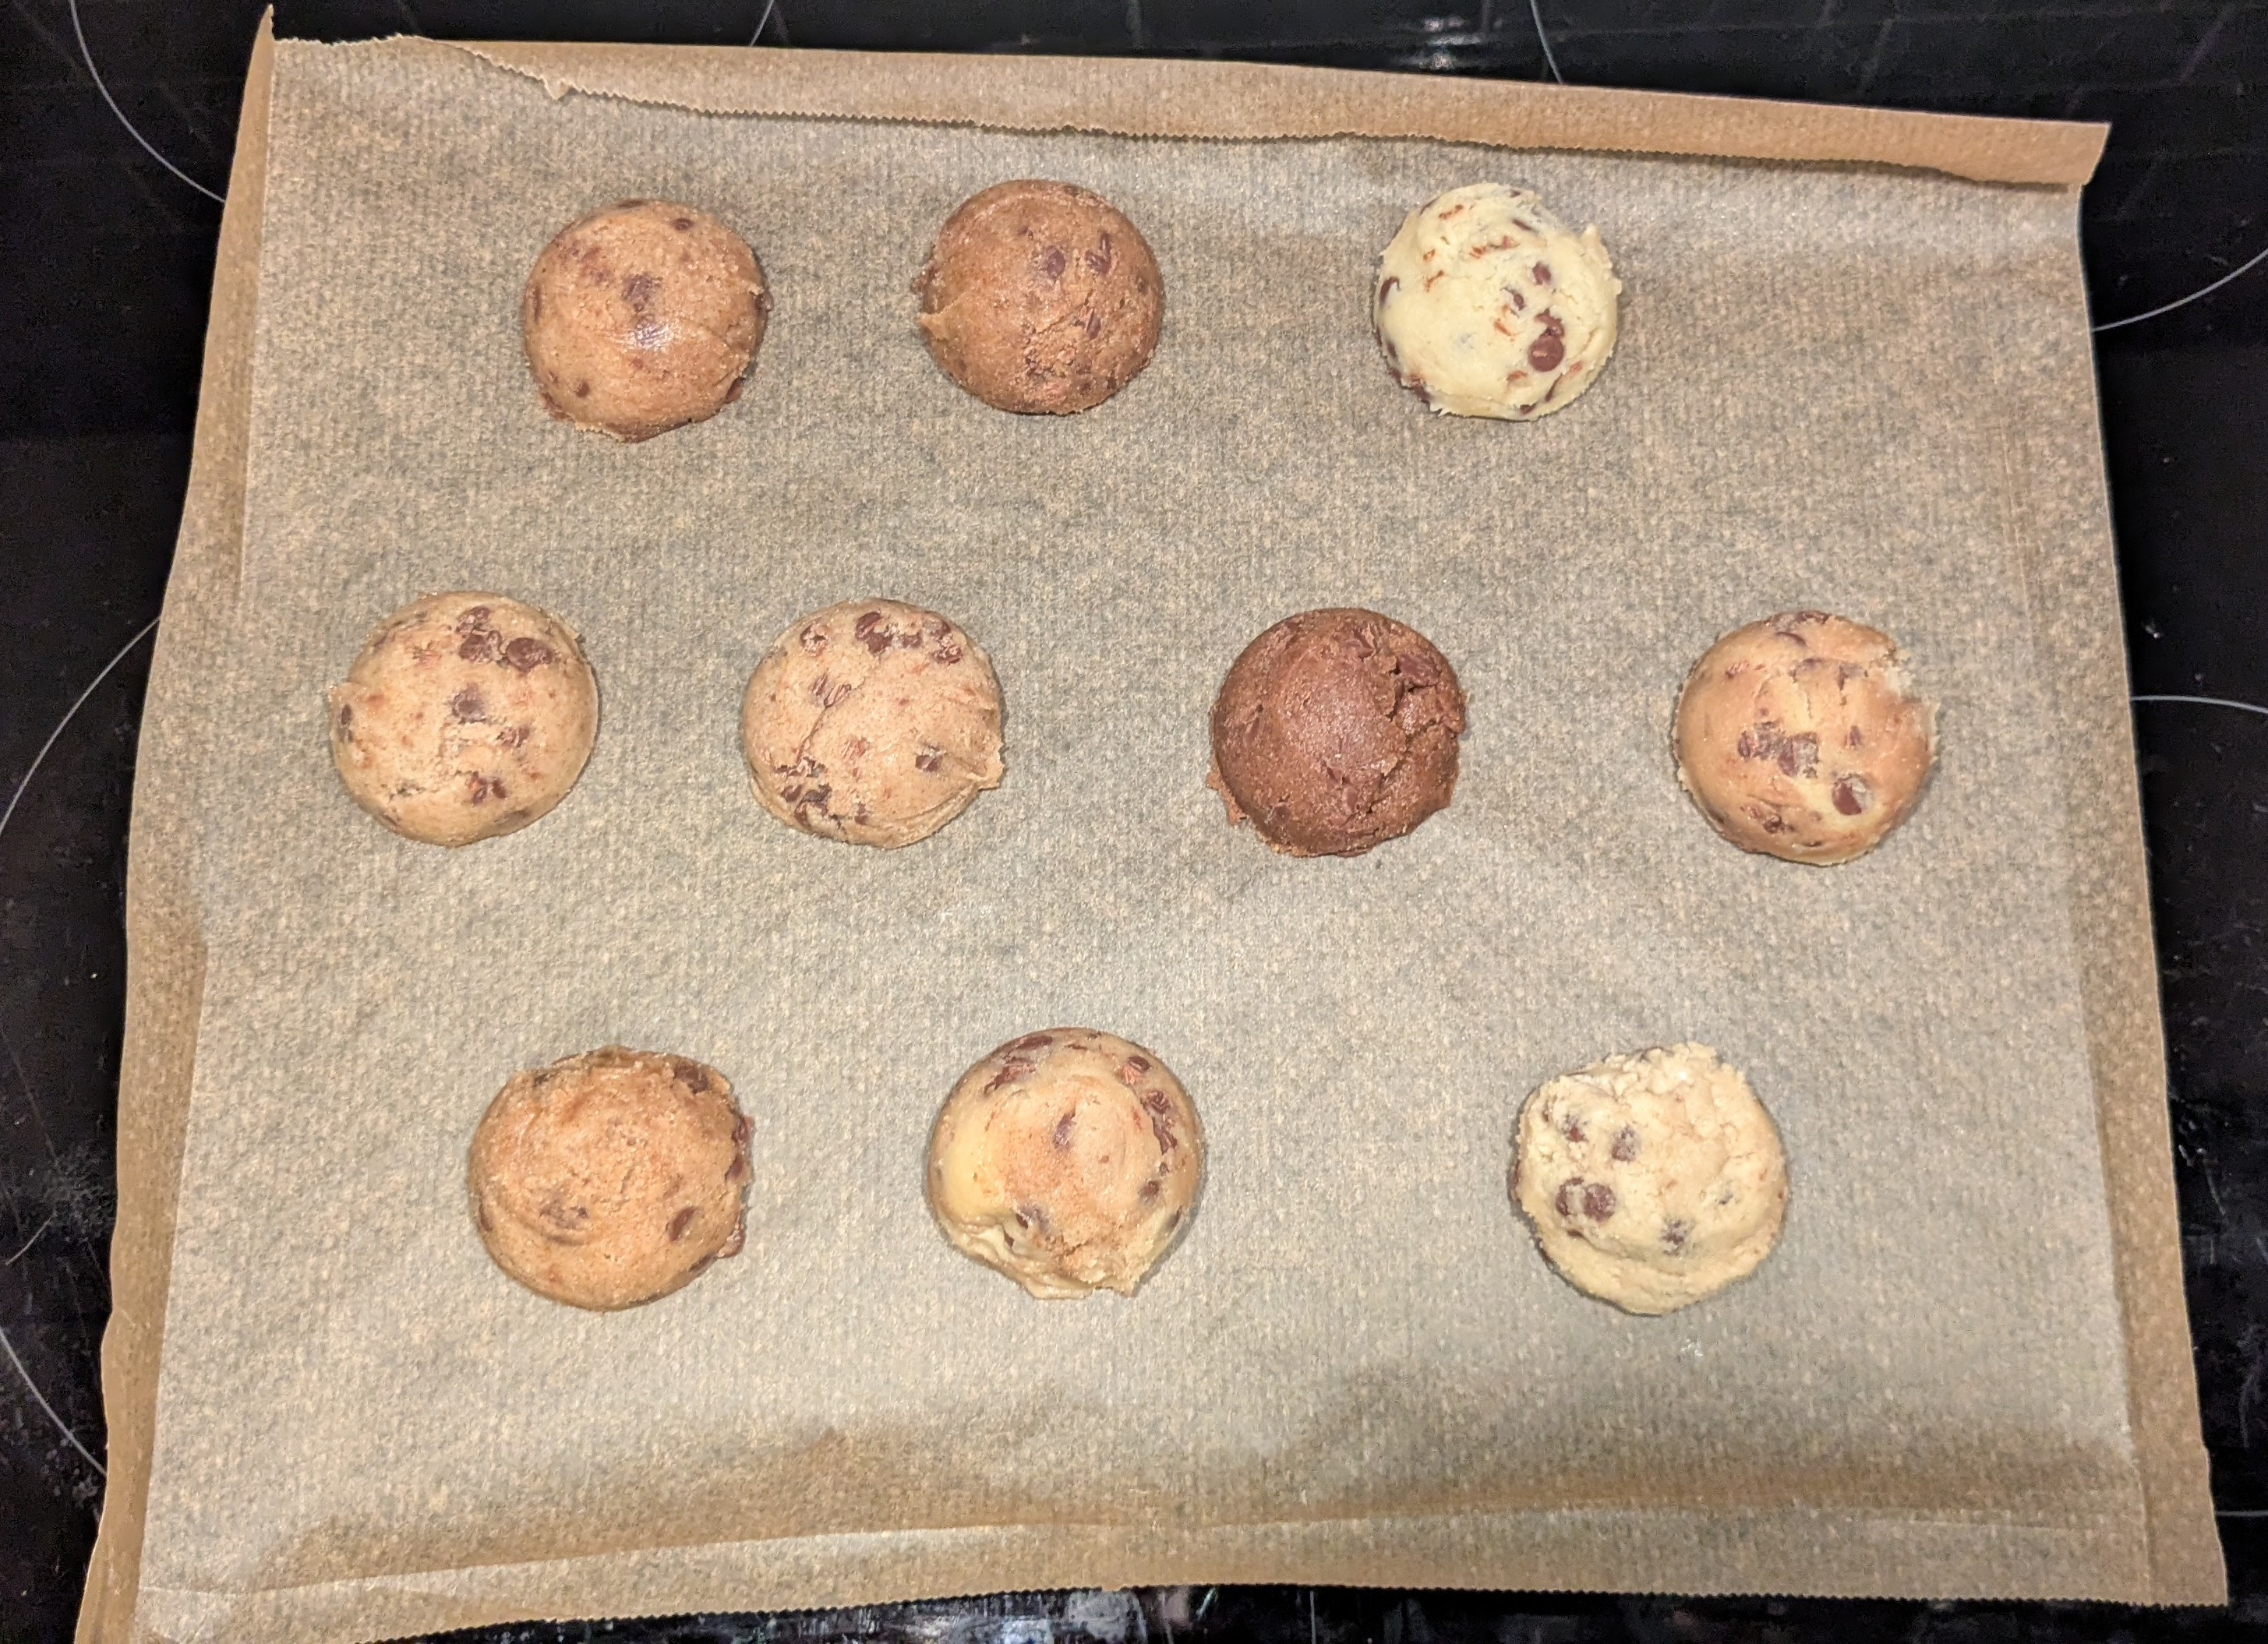
\includegraphics[width = \textwidth]{figures/block3_1_vorher.jpg}
\caption{Teigrohlinge vor dem Backen}
\label{fig:block3_1_vorher}
\end{subfigure}\hfill
\begin{subfigure}{0.49\textwidth}
\centering
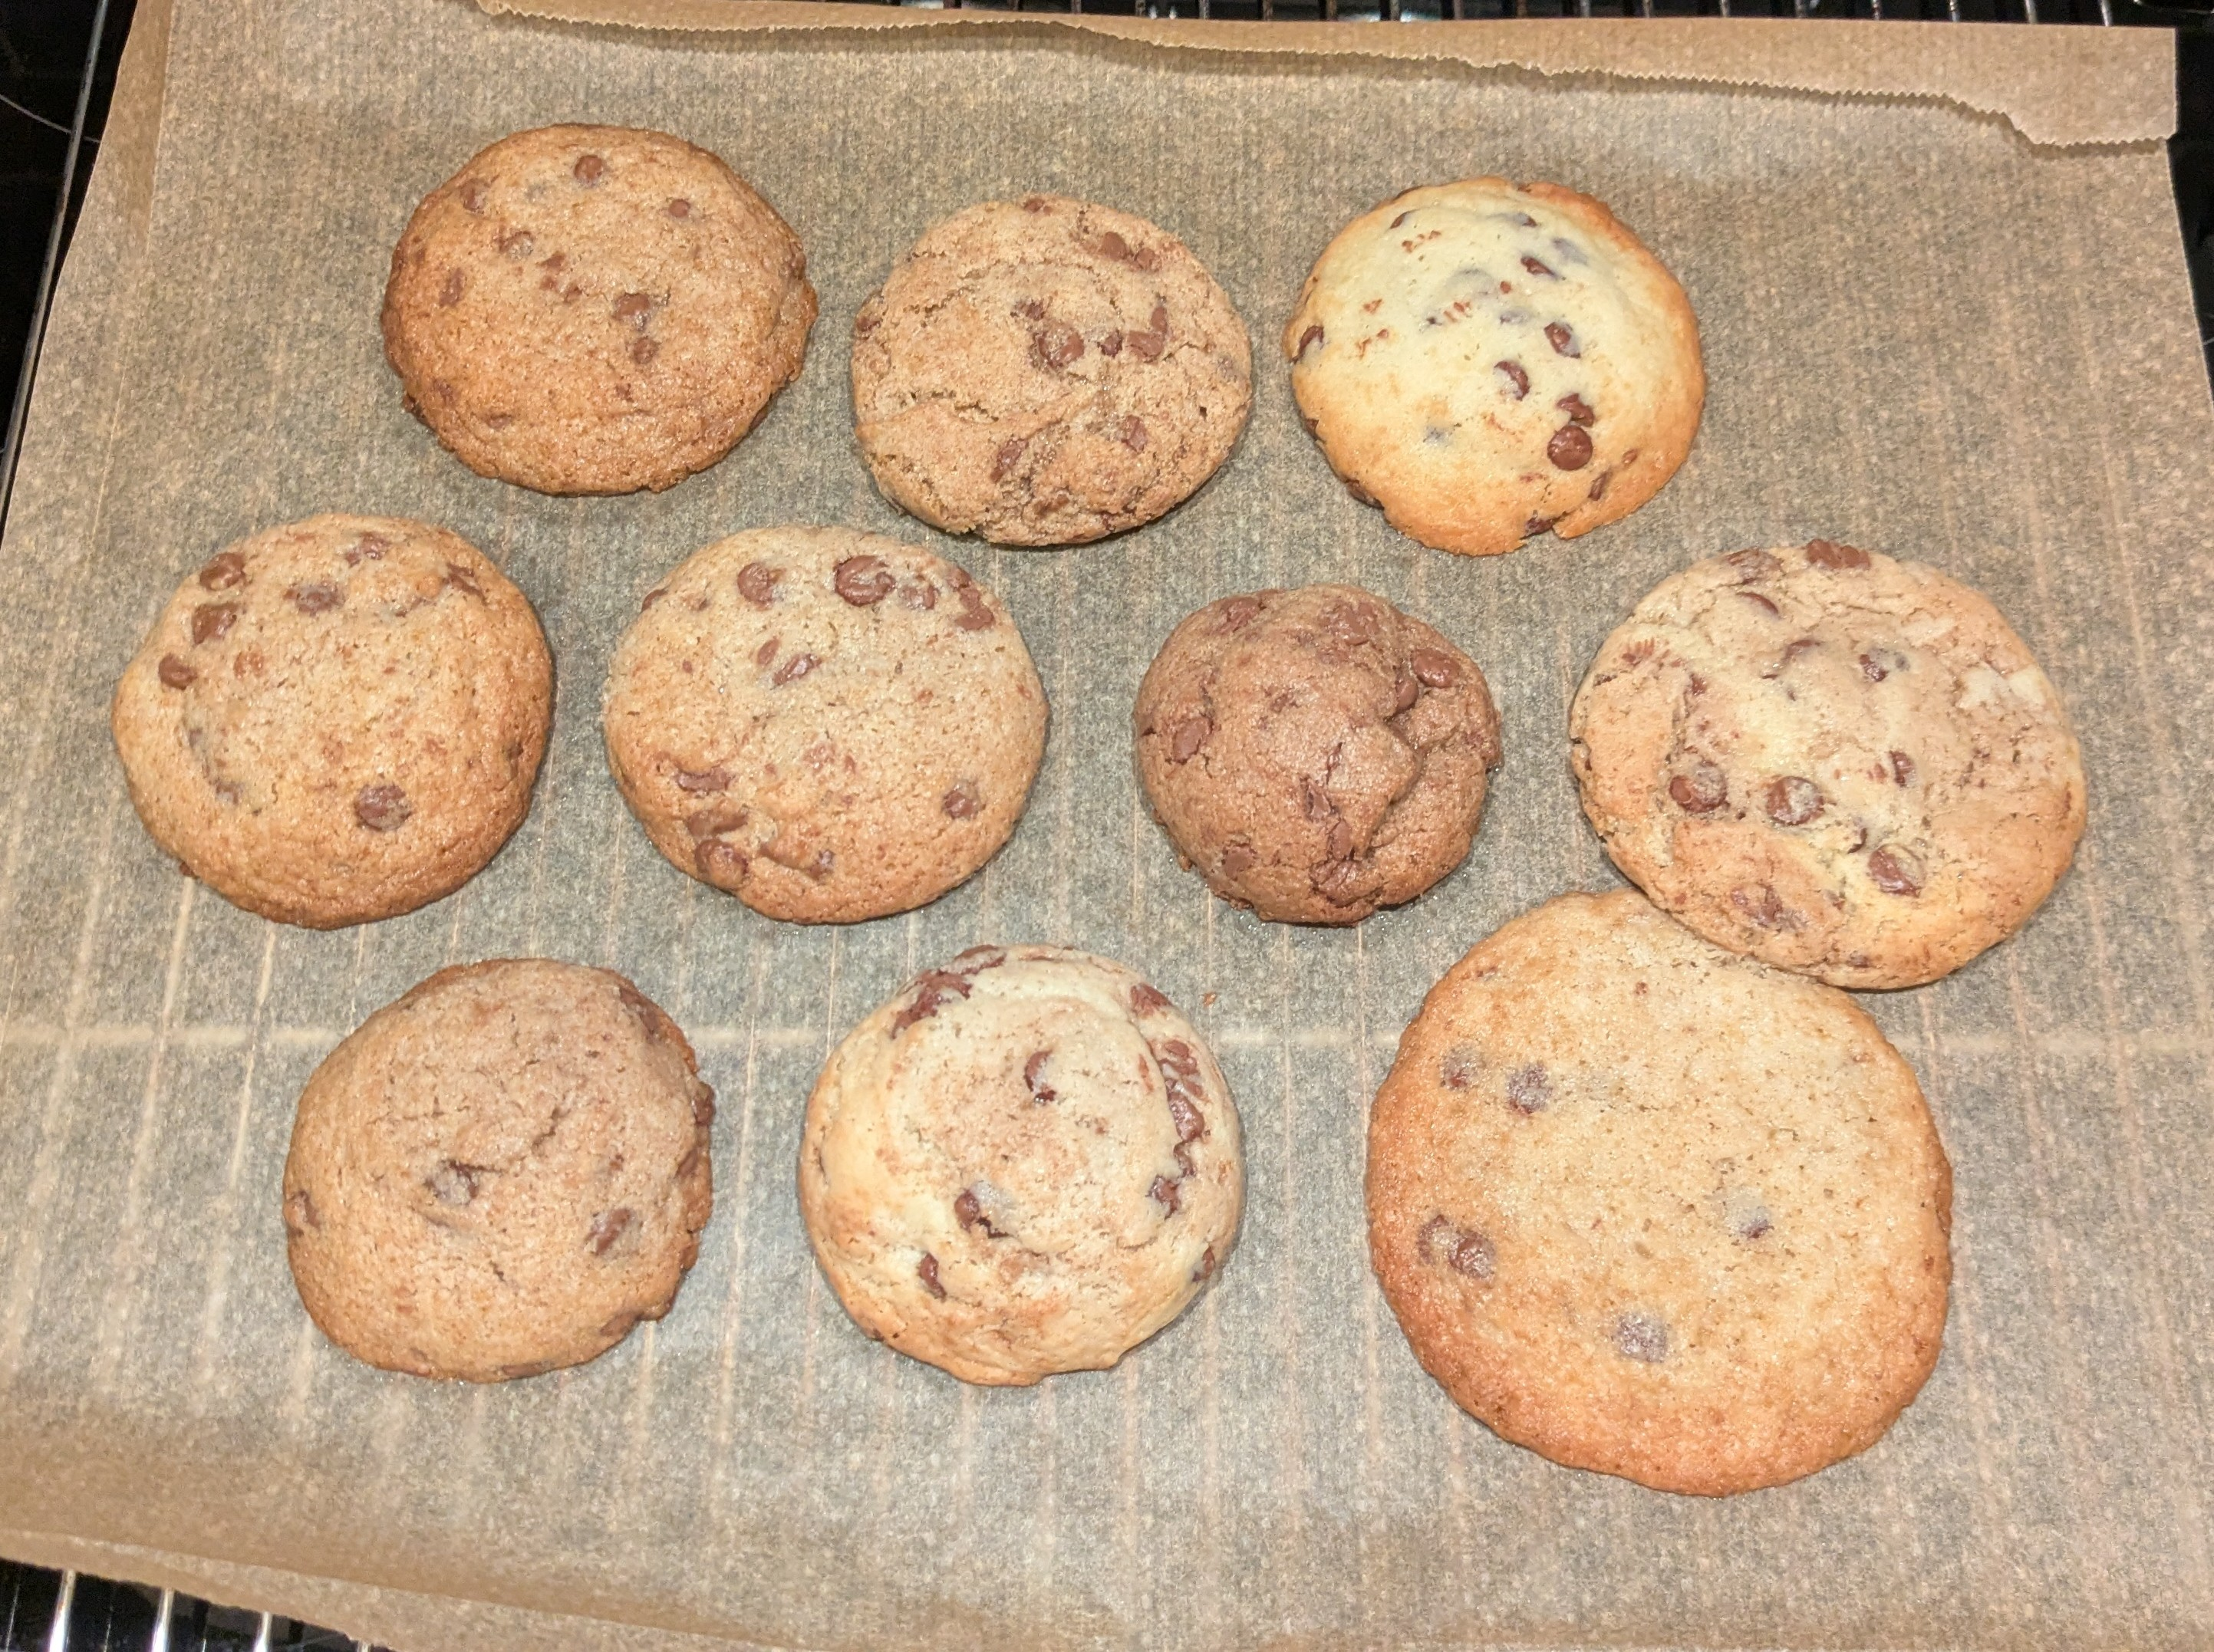
\includegraphics[width = \textwidth]{figures/block3_4_nachher.jpg}
\caption{Cookies nach dem Backvorgang}
\label{fig:block3_4_nacher}
\end{subfigure}
\caption{Backvorgang der dritten Replikation}
\label{fig:block_3}
\end{figure}